\documentclass[letterpaper, titlepage,openright, oneside,11pt]{book}
 %\documentclass[letterpaper,onepage,openright,titlepage,openany,oneside,11pt]{book}
\usepackage[T1]{fontenc}
\usepackage[latin1]{inputenc}
\usepackage{amsmath}
\usepackage{amsthm}
\usepackage{amsfonts}
\usepackage{amssymb}
\usepackage[spanish]{babel}
\usepackage[latin1]{inputenc}
\usepackage{graphicx}
\usepackage{amsmath}
\usepackage{dsfont} % colocar los numeros r
\usepackage{float}
\usepackage{fancyhdr}
\usepackage{anysize}
\usepackage{booktabs}
\usepackage{multirow}
\usepackage{titlesec}
\usepackage{enumerate}
\usepackage{verbatim}
%%%%%%%%%%%%%%%%%%%%
%\cxset{style7}
%Options: Sonny, Lenny, Glenn, Conny, Rejne, Bjarne, Bjornstrup
%\usepackage[Bjornstrup]{fncychap}

%%%%%%%%%

%pruebas




%%%%%%%%%%
\marginsize {3.8cm}{3.5cm}{4cm}{1.6cm}
\setlength{\paperheight}{24cm} \setlength{\paperwidth}{18cm}
\newtheorem{thm}{Teorema}[section]
\newtheorem{cor}[thm]{Corolario}
\newtheorem{defn}[thm]{Definici\'{o}n}
\newtheorem{ej}[thm]{Ejemplo}
\newtheorem{lem}[thm]{Lema}
\newtheorem{prop}[thm]{Proposici\'{o}n}
\def\bibname{Referencias}
\renewcommand{\contentsname}{Contenido}
\renewcommand{\baselinestretch}{1.1} 
 \renewcommand{\labelenumi}{\Roman{enumi}.} %interlineado
\def\chaptername{Cap\'{\i}tulo }
\decimalpoint

\bibliographystyle{apalike}
\begin{document}
%\documentclass[letterpaper, titlepage,openright, oneside,11pt]{book}
 %\documentclass[letterpaper,onepage,openright,titlepage,openany,oneside,11pt]{book}
\usepackage[T1]{fontenc}
\usepackage[latin1]{inputenc}
\usepackage{amsmath}
\usepackage{amsthm}
\usepackage{amsfonts}
\usepackage{amssymb}
\usepackage[spanish]{babel}
\usepackage[latin1]{inputenc}
\usepackage{graphicx}
\usepackage{amsmath}
\usepackage{dsfont} % colocar los numeros r
\usepackage{float}
\usepackage{fancyhdr}
\usepackage{anysize}
\usepackage{booktabs}
\usepackage{multirow}
\usepackage{titlesec}
\usepackage{enumerate}
\usepackage{verbatim}





\begin{document}




\thispagestyle{empty}

% Barra izquierda y escudo

% \hskip-0.5cm

%\vskip-0.5cm

% \vspace{-2.9cm}

\begin{minipage}[c][13cm][s]{3cm}
% \begin{minipage}[c][13cm][s]{0.3\textwidth}

    \begin{center}

        \includegraphics[height = 3.5cm]{logo_cimat.png} \\[13pt] %\color{vinoCimat}

        \hskip3pt \vrule width1pt height19cm
        \hskip1mm \vrule width2pt height19cm
        \hskip1mm \vrule width1pt height19cm \\[15pt]

    \end{center}

\end{minipage}
\begin{minipage}[c][11cm][s]{13.4cm}
% \begin{minipage}[c][11cm][s]{1.0\textwidth}
\vspace{8mm} \LARGE Centro de Investigaci\'on en Matem\'aticas,
A.C. \\    \begin{center}
     \vspace{.1cm}  %\color{vinoCimat}

        \hrule height1pt

        \vspace{.1cm}

        \hrule height2pt

        \vspace{.1cm}

        \hrule height1pt

        \vspace{2.2cm}

%Define el t\'itulo, autor y fecha

% \title

%       \color{black}


       {
     \vspace{-3mm} \LARGE  \textbf{CONFIABILIDAD Y ALGUNAS POL\'ITICAS DE INVENTARIO EN TRANSFORMADORES DE INSTRUMENTO. }\\

\vspace{8mm} \LARGE \textbf{T E S I S }\\

      }

% \author

      { \vspace{5mm}\LARGE

                       \textbf{Que para obtener el grado de:}\\

            \vspace{5mm}      {Maestro en Ciencias con Especialidad en}\\

                       {Probabilidad y Estad\'istica}\\

     \vspace{13mm}           P  R  E  S  E  N  T  A \\

     \vspace{5mm}     \textbf{Alma Delia Maldonado Santiago}\\

     \vspace{13mm}      {DIRECTORES DE TESIS:} \\

     \vspace{5mm}     {\textbf{Dr. Enrique Ra\'ul Villa Diharce} }\\
     
       \vspace{5mm}     {\textbf{ Dr. Jos\'e Andr\'es Christen Gracia} }\\

     \vspace{13mm}

      }

%       \date{\today}

     \LARGE{Guanajuato, Gto.                                Agosto del 2013}

    \end{center}

\end{minipage}

\newpage

\end{document}

\renewcommand{\tablename}{Tabla}
\frontmatter
\thispagestyle{empty}
%\title{\bf Confiabilidad y algunas pol\'iticas de inventario en transformadores de instrumento.}
%\author{Maldonado Santiago Alma Delia}
%\maketitle
 %\newpage{\pagestyle{empty}
% \cleardoublepage} 

%\begin{flushright}
%\vskip5cm \sc{Dedicatoria}\\
%
%
%
%A mis padres\\
%
%Pedro y Maria.\\
%
%Por que a ellos \\
%les debo todo lo que soy.
%\end{flushright}




\pagestyle{empty}

\noindent \mbox{{\huge \textbf{Dedicatoria}}}


\vspace{2cm}

%\begin{center}
\noindent
\begin{tabular}{p{13.2cm}}
\hline \hline

\medskip

A mis padres\\

Pedro Virgilio y Maria Teresa.\\

Por su apoyo incondicional en todos los momentos de mi vida.


\medskip
\end{tabular}





\newpage \thispagestyle{empty} \cleardoublepage




\noindent \mbox{{\huge \textbf{Agradecimientos}}}
\vspace{2cm}




\noindent
\begin{tabular}{p{13.2cm}}


\hline \hline

\\[0.3cm]
Mi m\'as sincero agradecimiento es para el Dr Enrique Villa Diharce y Dr. Andr\'es Christen Garc\'ia por haber compartido conmigo parte de su amplio
conocimiento en la realizaci\'on de esta tesis. 
\medskip


\indent A mis padres Pedro Virgilio Maldonado Mart\'inez  y Maria Teresa Santiago Ruiz les agradezco sus consejos, su
gu\'ia, su confianza en la realizaci\'on de mis sue\~nos y sobre todo su apoyo incondicional en todo momento. 
\medskip

\medskip
\indent A los buenos amigos que conoc\'i en esta etapa de mi vida, con quienes compart\'i grandes momentos y que son ahora parte de mi vida. En especial a Bryan Yaset Aguero Cruz por sus consejos, cari\~no y apoyo incondicional brindados durante mi estancia en Guanajuato.
\medskip

\indent Agradezco al CONACYT por el apoyo recibido en la realizaci\'on de mis estudios de maestr\'ia, al CIMAT, A. C. por la gran oportunidad que represent\'o en mi desarrollo profesional.
\end{tabular}


\newpage \thispagestyle{empty} \cleardoublepage

\tableofcontents
\newpage
\pagestyle{fancy}
\fancyhf{} % delete current setting for header and footer
\fancyhead[LE,RO]{\bfseries\thepage}
%
\fancyhead[LO]{\bfseries\rightmark}%
\fancyhead[RO,LE]{\thepage} % N�meros de p�gina en las esquinas de los encabezados


\mainmatter
\addcontentsline{toc}{chapter} {Introducci\'on}


%\addcontentsline{toc}{chapter} {Introducci\'on}

%
%\documentclass[letterpaper, titlepage,openright, twoside,11pt]{book}
%\usepackage[latin1]{inputenc}
%\usepackage{amsmath}
%\usepackage{amsthm}
%\usepackage{amsfonts}
%\usepackage{amssymb}
%\usepackage[spanish]{babel}
%\usepackage[latin1]{inputenc}
%\usepackage{graphicx}
%\usepackage{amsmath}
%\usepackage{dsfont} % colocar los numeros r
%\usepackage{float}
%\usepackage{fancyhdr}
%\usepackage{anysize}
%\decimalpoint
%\begin{document}
%\renewcommand{\tablename}{Tabla}
\chapter*{Introducci\'on}
\noindent  La estad\'istica Bayesiana es hoy en d\'ia  ampliamente usada, en parte debido a la flexibilidad de incluir informaci\'on conocida previamente. En los \'ultimos a\~nos el estudio de confiabilidad dentro del \'ambito industrial ha tomado gran importancia, al describir los tiempos de vida y evaluar el desgaste de sus instrumentos de trabajo utilizados. En el presente trabajo se conjugan estas dos \'areas, para  proponer un plan de inventario \'optimo de los transformadores de instrumento empleados en las subestaciones de Veracruz, empleando una funci\'on de utilidad. A continuaci\'on se da un panorama general del contenido de este trabajo.


\noindent Para introducir al lector en el contexto de inter\'es, en el cap\'itulo 1 se proporciona la descripci\'on del problema, junto con los objetivos generales del trabajo.\\[0.1cm]
\noindent En el cap\'itulo 2, se comentan los principales resultados utilizados  en la teor\'ia de  confiabilidad. Se da una breve introducci\'on al uso de m\'etodos Bayesianos y la manera de realizar inferencia y estimaci\'on. Los principales m\'etodos computacionales empleados para la obtenci\'on de la distribuci\'on posterior, son explicados de manera general dentro de este cap\'itulo.\\[0.1cm]
\noindent En el cap\'itulo 3, se ver\'a la manera de analizar los datos de transformadores de instrumento dentro de un enfoque Bayesiano.
Empezando  con la propuesta de la distribuci\'on a priori de los tiempos de vida y la manera detallada de establecerse, para continuar con encontrar la distribuci\'on posterior. Debido a que esta \'ultima result\'o ser una expresi\'on compleja, se recurri\'o al empleo de m\'etodos computacionalmente intensivos, para la obtenci\'on de un muestra de la distribuci\'on posterior. Posteriormente las funci\'ones de confiabilidad y riesgo son ilustradas empleando esta muestra.

\noindent  Al inicio del cap\'itulo 4, se hace un breve resumen de la informaci\'on relevante del cap\'itulo 3, que ayudar\'a al establecimiento de la funci\'on de utilidad. Primero se describe la construcci\'on de distintas funciones de utilidad, junto con sus utilidades esperadas y  se detalla la manera de obtener aproximaciones para estas funciones. Al final del cap\'itulo se describen las conclusiones y comparaciones entre las distintas utilidades esperadas.
%Despu�s haciendo algunos supuestos, sobre la forma de operar del almac\'en, se realizan simulaciones. Las simulaciones permiten crear una imitaci\'on de la evoluci\'on el n\'umero de transformadores en el almac\'en a lo largo del tiempo. Con este m\'etodo se determina la cantidad adecuada de transformadores almacenados que deber\'ian tenerse.

\noindent Posteriormente el cap\'itulo 5, contiene conclusiones generales y trabajos a futuro. Finalmente se aportan los c\'odigos en R, empleados para realizar las simulaciones y la distribuci\'on a priori.

\newpage \thispagestyle{empty} \cleardoublepage

%\end{document}








%%
%\documentclass[letterpaper, titlepage,openright, twoside,11pt]{book}
%\usepackage[latin1]{inputenc}
%\usepackage{amsmath}
%\usepackage{amsthm}
%\usepackage{amsfonts}
%\usepackage{amssymb}
%\usepackage[spanish]{babel}
%\usepackage[latin1]{inputenc}
%\usepackage{graphicx}
%\usepackage{amsmath}
%\usepackage{dsfont} % colocar los numeros r
%\usepackage{float}
%\usepackage{fancyhdr}
%\usepackage{anysize}
%\decimalpoint
%\begin{document}
%\renewcommand{\tablename}{Tabla}

%\addcontentsline{toc}{chapter} {Elementos Generales de confiabilidad}
%%%%%%%%%%%%%%%%%%%%%%%%%%%%%%%%%%%%
\chapter{Objetivos}

\section{Definici\'on del problema}

\noindent En el 2006 los transformadores de instrumento en las  sub\'areas de Coatzacoalcos y Temascal (Veracruz), observaron un n\'umero inusualmente elevado de fallas, lo que condujo a la necesidad de estudiar la confiabilidad de los transformadores. Se deseaba pronosticar el n\'umero de fallas de sus equipos  por a\~no. En el estudio realizado por el CIMAT, se hizo un an\'alisis de los datos disponibles, empezando por un an\'alisis exploratorio. Posteriormente realizaron distintas comparaciones por tipo, estatus y marca de los transformadores, para  finalmente centrarse en el estudio de los transformadores con m\'as fallas, que resultaron ser los transformadores de corriente. \\[0.1cm]
\noindent Al realizar el an\'alisis de confiabilidad se obtuvo que la distribuci\'on que mejor ajustaba a los datos es una distribuci\'on  Weibull. Bajo esta distribuci\'on se estimaron los par\'ametros, algunos cuantiles de inter\'es e intervalos de confianza usando la aproximaci\'on normal. Adem\'as se analiz\'o el estado de las unidades que sobrevivieron a un tiempo determinado, mediante la funci\'on de riesgo y la confiabilidad condicional, con la finalidad de pronosticar las tasas de falla de los transformadores.\\[0.1cm]

\noindent El inter\'es de este trabajo radica en realizar un an\'alisis de confiabilidad desde el enfoque Bayesiano, hacer estimaciones de las funciones de confiabilidad y describir la tasa de desgaste de las unidades. Esto conducir\'a a proponer una pol\'itica adecuada que minimice los costos de almacenamiento de los equipos, mediante una funci\'on de utilidad, para pronosticar el n\'umero de transformadores requeridos en el almac\'en hasta un tiempo espec\'ifico.


\section{Justificaci\'on}

\noindent Actualmente una de las mayores necesidades de una empresa o negocio, es el empleo \'optimo de sus herramientas de trabajo. Una falla en sus instrumentos implica p\'erdidas en mayor o menor medida. As\'i el implementar pol\'iticas \'optimas y planes estrat\'egicos de sus herramientas de uso, ha significado una parte crucial en el desempe\~no de su trabajo.\\
\noindent Por lo tanto, el generar un plan de inventario para los transformadores resultar\'a de gran importancia. Dado que los transformadores de instrumento son costosos, resultar\'a  \'util estimar su tiempo de vida. \\
%En particular los costos que se  analizar\'an son los siguientes:
%\begin{itemize}
%\item El costo de almacenamiento de los transformadores que no son usados en un periodo dado pero est\'an disponibles en el almac\'en.
%\item El costo de no poder cobrar la electricidad durante un periodo donde no hab\'ia un transformador en reserva.
%\end{itemize}

\noindent La presente investigaci\'on se justifica desde dos puntos de vista:
\begin{itemize}
\item Desde el punto de vista pr\'actico, se desea proponer al problema planteado una estrateg\'ia de acci\'on, empleando funciones de utilidad que permitan minimizar los costos esperados.
\item Desde el punto de vista te\'orico, esta investigaci\'on generar\'a reflexi\'on y discusi\'on sobre el conocimiento existente, en cuanto a la forma de comportarse de los transformadores.
\end{itemize}

\noindent Dentro del desarrollo de esta tesina se har\'a lo siguiente:

\begin{enumerate}
\item Revisar la teor\'ia Bayesiana necesaria para abordar el problema.
\item Proponer alguna estrategia \'optima de inventario o almacenamiento, mediante una funci\'on de utilidad que permita minimizar los costos esperados. 

\end{enumerate}
\noindent A continuaci\'on mencionaremos que son los transformadores de instrumento, y en que radica la importancia en desarrollar un plan \'optimo de inventario.


\section{Transformadores de Instrumento}

\noindent Un transformador el\'ectrico utiliza las propiedades f\'isicas de la inducci\'on electromagn\'etica y es capaz de elevar o disminuir la tensi\'on el\'ectrica, transformar la frecuencia, equilibrar o desequilibrar circuitos el\'ectricos, seg\'un la necesidad y caso espec\'ifico.\\
\noindent El primer transformador fue construido por Michael Faraday, compuesto por dos bobinas enrolladas una encima de la otra. Al variar la corriente que circulaba en una de ellas, cerrando o abriendo el interruptor, el flujo magn\'etico a trav\'es de la otra bobina variaba, y se induc\'ia una corriente el\'ectrica.\\[0.1cm]
\noindent A partir de entonces se han creado diferentes tipos de transformadores cada vez m\'as sofisticados, pero empleando el mismo principio de inducci\'on. En particular en esta tesina se utilizar\'an un tipo especial de transformadores, llamados transformadores de instrumento.\\[0.1cm]
%flujo electromagn�tico, es la medida o cantidad de magnetismo, considerando la intensidad y la extensi�n de un campo magn�tico, un campo magn�tico es un campo de fuerzas que existe alrededor de un campo cuerpo magn�tico o de un conductor que transporta corriente. 
\noindent Los transformadores de instrumento (TI) tienen la tarea de convertir grandes valores de corriente y voltaje a valores peque\~nos que son f\'acilmente aplicables, para los prop\'ositos de medici\'on y protecci\'on. Su misi\'on es evitar la presencia de elevadas tensiones en aquellos dispositivos que van a estar al alcance de las personas. Estos transformadores pueden ser de dos tipos:
\begin{itemize}
\item Transformador de potencial(TP): Cuya funci\'on es transformar o cambiar el voltaje, com\'unmente se enfocan en reducir el voltaje. %,es decir, modera la fuerza con que se mueven los electrones.
\item Transformador de corriente (TC): Su funci\'on consiste en transformar o cambiar la corriente.
%es decir, se encargan de cambiar la cantidad de electrones  que circulan en un determinado momento.
\end{itemize}


%
%Las principales razones por las que se usan los transformadores de instrumento son 
%\begin{itemize}
%\item Para reducir en forma precisa, por medio de la relaci\'on de transformaci\'on, la magnitud de la corriente o voltaje del circuito primario a valores mas manejables en el circuito secundario. Por lo general la salida del secundario a 115 o 120 Volts en el TP y 5 a 1 Amp en el TC.
%\item Para aislar el equipo secundario (instrumentos de medici\'on y de protecci\'on) del voltaje primario, que por su valor los da\~naria.
%\end{itemize}

 \begin{figure}[h!]
\begin{center}
\includegraphics[scale=0.8]{trans.jpg}
\end{center}
\vspace{-.5 cm} \caption{\bf Transformadores de medici\'on.}\label{tranF}
\end{figure}

\noindent Los transformadores resultan de suma importancia en la generaci\'on y distribuci\'on de la energ\'ia el\'ectrica. Su inter\'es principal radica en los siguientes puntos: 

\begin{itemize}
\item Los transformadores de instrumento (Figura\ref{tranF}), ayudan a determinar los consumos de energ\'ia, formando parte del sistema de medici\'on de energ\'ia el\'ectrica para las redes de alta tensi\'on y con ellos realizar los montos de los  cobros. En la parte superior del transformador se conecta la red el\'ectrica. Mientras que en la parte inferior se colocan los elementos de medici\'on, en esta parte la tensi\'on el\'ectrica es mucho m\'as reducida que en la superior.
\item Sirven de protecci\'on, al momento en que se origina una descarga. El sistema designado para protecci\'on desactiva los interruptores, con lo que evita que se generen da\~nos de mayor magnitud en la red.
\item Cuando el transformador falla de manera catastr\'ofica impide la medici\'on del flujo de energia el\'ectrica.
\end{itemize}
\noindent  La falta de alguno de ellos implica p\'erdidas econ\'omicas para la empresa que proveer el servicio de energ\'ia . Sin embargo el tener demasiados en almac\'en implica p\'erdidas tambi\'en. Lo ideal es encontrar  una cantidad adecuada de transformadores, de tal forma que los costo sean m\'inimos, esto es debemos optimizar el inventario.

  

   
  
%  
%  La energ\'ia el\'ectrica en tiempo real son sistemas que sumistran energ\'ia. En tiempo real significa que e la energ\'ia es generada, transformada y suministrada al momento 
%

\newpage \thispagestyle{empty} \cleardoublepage







%\end{document} 

\chapter{Conceptos B\'asicos}
\noindent En  estad\'istica industrial el \'area de confiabilidad es una rama ampliamente utilizada.
Su origen se remonta a  la d\'ecada de los a\~nos 40, en aplicaciones militares durante la segunda guerra mundial. Fue empleada para estudiar el funcionamiento de equipos electr\'onicos y mec\'anicos  por periodos largos de tiempo. A partir de entonces esta rama se ha empleado dentro de empresas y negocios para la evaluaci\'on de la confiabilidad de sus componentes.\\[0.1cm]
\noindent  D\'ia con d\'ia la competencia entre productos y servicios proporcionados por empresas hacen que estas  se preocupen por la durabilidad de sus productos, pero al mismo tiempo la optimizaci\'on de sus costos. En un estudio de confiabilidad se pueden evaluar y cuantificar estos aspectos.

\noindent Desde el surgimiento de la rama de confiabilidad se han propuesto distintas definiciones, a continuaci\'on mencionaremos dos de ellas:

\begin{itemize}
\item  La confiabilidad es la probabilidad de que una unidad realice su funci\'on hasta un tiempo espec\'ifico bajo las condiciones de uso encontradas.$[{\bf \ref{me}}]$
\item La confiabilidad se refiere al funcionamiento adecuado de equipos y sistemas en el cual influye factores como software, hardware, humanos y ambientales, es decir, la probabilidad que algo funcione exitosamente bajo condiciones espec\'ificas como funci\'on del tiempo.$[{\bf \ref{law}}]$
\end{itemize} 
\noindent  Existen muchas otras expectativas de lo que deber\'ia ser  confiabilidad, pero todas ellas enfatizan, a que confiabilidad se refiere, a la calidad que tiene un sistema a trav\'es del tiempo, e involucra elementos que conllevan al mejoramiento, pron\'ostico y mantenimiento del sistema, es decir, que funcione de manera correcta durante el tiempo que sea usado y bajo las condiciones para las cuales fue creado. \\[0.2cm]


\noindent El principal an\'alisis en confiabilidad se centra en  periodos para los cuales el componente funciona, lo que com\'unmente son llamados tiempos de vida o tiempos a la falla. 

\noindent Por ejemplo, supongamos que se desea hallar la confiabilidad de  maquinas de cocer que laboran 8 horas al d\'ia. Se  observan $n$ maquinas de cocer durante un periodo de tiempo y se registran los tiempos en que fallaron o dejaron de funcionar, es decir, los tiempos de vida o 
 tiempos a la falla. Supongamos adem\'as que de las  $n$ maquinas solo $k$   maquinas fallaron y $n-k$ no fallaron, al finalizar el periodo de observaci\'on. Esta informaci\'on es proporcionada para realizar un estudio de confiabilidad. Un punto importante a recalcar es que debido a que siempre se tienen limitantes de tiempo al momento de observar el funcionamiento de componentes, es muy com\'un trabajar con datos censurados. En este contexto un dato censurado ser\'a aquella observaci\'on que nos da informaci\'on parcial de las ocurrencias de las fallas. Existen tres tipos principales de censura:
\begin{itemize}
\item Censura por la derecha: Se fija un tiempo de observaci\'on y las unidades que no fallaron son llamados censuras por la derecha.

\item Censura por la izquierda: Ocurre cuando al inspeccionar las unidades despu\'es de un periodo de tiempo se encuentra que algunas ya fallaron, pero no se sabe el momento de su ocurrencia.
\item Censura por intervalo: Cuando se inspecciona en intervalos de tiempo y se observan fallas en cierto intervalo pero no se conoce exactamente en que momento ocurrieron.
\end{itemize}



\noindent Teniendo claro que los tiempos de vida son los datos registrados del tiempo de funcionamiento de un  componente, es com\'un preguntarse la manera en que se modelan estos tiempos.  Los tiempos de vida son observaciones aleatorias que var\'ian a trav\'es del tiempo, por lo tanto son modelados por variables aleatorias. 
%Una variable aleatoria se define de la siguiente manera: 
%
%%El an\'alisis de tiempos de vida envuelve una an\'alisis de cuantiles positivos y continuos, que son los tiempos de vida para el cual el componente funciona.\\[0.2cm]
%%Los  tiempo de vida son representados por variables aleatorias:
%
%
%
%\begin{defn} 
%Sea $(\Omega, F, P)$ un espacio de probabilidad y sea $X:\Omega\rightarrow \mathbb{R}$ una funci\'on tal que $X^{-1}((-\infty,x])=\{\omega|X(\omega)\leq x\}\in F$ para todo $x$. Entonces $X$ se llama variable aleatoria.
%\end{defn}
%
%\noindent Al emplear variables aleatorias existen ciertas funciones que las caracterizan. Algunas de ellas son la funci\'on de densidad, distribuci\'on acumulada, confiabilidad y riesgo, entre otras, de las cuales podemos obtener informaci\'on valiosa acerca del fen\'omeno que se esta modelando.
%
%\begin{defn}
%Si $X$ es una variable aleatoria, la funci\'on $F:\mathbb{R}\rightarrow\mathbb{R}$ definida por $$F(x)=P(X\leq x).$$ Se llama funci\'on de distribuci\'on acumulada de $X$. Toda funci\'on de distribuci\'on satisface lo siguiente:
%\begin{enumerate}
%\item$F$ es mon\'otona y creciente.
%\item $F$ es continua por la derecha y tiene l\'imites por la izquierda.
%\end{enumerate}
%\end{defn}
%
%\noindent Existen dos tipos importantes de distribuciones: discretas y continuas.
%\noindent Para una variable aleatoria discreta $X$ definida sobre un espacio muestral $S$, la funci\'on de probabilidad satisface:
%$$P(X=x)=P(x)\geq 0,\mbox{   } x\in S,$$
%$$\sum_{x\in S} P(x)=1.$$
%
%\noindent Mientras que para una variable aleatoria continua, la funci\'on de densidad de probabilidad (fdp) esta definida como  $f:\mathbb{R}\rightarrow\mathbb{R^{+}}$ cumple:
%$$f(x)\geq 0 ,$$
%$$\int_{-\infty}^{\infty} f(x) dx=1.$$
%
%\noindent El  $p$-\'esimo cuant\'il de una variable aleatoria  $X$ es el valor $t_p$ tal que 
%$$P(X\leq t_p)=p.$$ Donde $t_p=F^{-1}(p)$. Para los tiempos de falla, $t_p$ es el tiempo al cual el 100$p\%$ de las unidades o componentes fallar\'an.[{\bf\ref{me}}]\\[0.2cm]
\noindent Dentro del an\'alisis de confiabilidad la funci\'on principal que se usa para estudiar los tiempos de vida es la funci\'on de confiabilidad.\\[0.1cm]
\noindent Si $T$ una variable aleatoria entonces la funci\'on de confiabilidad o supervivencia esta dada por:
\begin{eqnarray}\label{confiabi}
 C(t)=P(T>t)=1-F(t).
\end{eqnarray}


\noindent Donde $F$ es la funci\'on de distribuci\'on acumulada de la variable aleatoria $T$. La ecuaci\'on (\ref{confiabi})  calcula la probabilidad de que una unidad sobreviva despues de un tiempo $t$. 
\noindent La funci\'on que analiza la tasa de falla instant\'anea o la manera en la cual un componente se degrada es la funci\'on de riesgo.\\[.1cm]
Supongamos que estamos interesados en la probabilidad de que un componente que ha trabajado hasta un tiempo $t$, falle en un intervalo  $[t,t+\Delta t]$, es decir,  
\begin{eqnarray*}
P(t<T\leq t+\Delta t |T>t) =\frac{P(t<T \leq t+\Delta t )}{P(T>t)}=\frac{F(t+\Delta t )-F(t)}{C(t)}
\end{eqnarray*}


\noindent  Si deseamos conocer su tasa de falla, entonces tendremos que dividir entre la longitud del intervalo y hacerlo tender a cero, es decir,
 
\begin{eqnarray*}
h(t)&=&\lim_{\Delta t \rightarrow 0}\frac{P(t<T\leq\Delta t |T>t)}{\Delta t }\\
&=&\lim_{\Delta t \rightarrow 0}\frac{F(t+\Delta t)-F(t)}{\Delta t }\frac{1}{C(t)}\\
&=&\frac{\frac{d}{dt}F(t)}{C(t)}\\
&=&\frac{f(t)}{C(t)}
\end{eqnarray*} 
Por lo tanto la funci\'on de riesgo esta dada por:  $$h(t)=\frac{f(t)}{C(t)}.$$

\noindent Es importante ahora mencionar que dentro de la teor\'ia de confiabilidad existe una serie de distribuciones que com\'unmente se usan para modelar los tiempos de vida de los componentes. Las distribuciones m\'as comunes son la distribuci\'on Exponencial, distribuci\'on Weibull, distribuci\'on Lognormal, distrbuci\'on Log\'istica, distribuci\'on Gamma y distribuci\'on Gaussiana Inversa. La descripci\'on de ellas puede verse en {\bf [\ref{distribuciones}]}. Sin embargo en el desarrollo de esta tesina ser\'a de inter\'es considerar la distribuci\'on Weibull como veremos en cap\'itulos posteriores.
\section{Distribuci\'on Weibull}
\noindent La distribuci\'on de probabilidad Weibull fue propuesta por Waloddi Weibull  en 1951, para describir la fatiga de materiales. Hasta nuestros d\'ias es una distribuci\'on muy com\'un dentro del estudio de tiempos de vida.\\[0.1cm]
\noindent Se dice que una variable aleatoria $X$ tiene distribuci\'on Weibull, denotada como $X\sim$ Weibull$(\eta,\beta )$, si su funci\'on de densidad esta dada por:

\begin{eqnarray*}
f(t;\eta;\beta)=\frac{\beta}{\eta}\left(\frac{t}{\eta}\right)^{\beta-1}\exp\left\{-\left(\frac{t}{\eta}\right)^{\beta}\right\}
\end{eqnarray*}

\noindent donde $t>0,\beta>0$ y $\eta>0.$
\begin{figure}
\begin{center}
\includegraphics[scale=0.35]{weD.pdf}
\end{center}
\vspace{-1cm}\caption{\bf Comportamiento de la  densidad Weibull.}\label{wed}
\end{figure}

Entonces 

\begin{itemize}
\item Su funci\'on de distribuci\'on esta dada por:

\begin{eqnarray*}
F(t;\eta;\beta)=1-\exp\left\{-\left(\frac{t}{\eta}\right)^{\beta}\right\}
\end{eqnarray*}

\begin{figure}
\begin{center}
\includegraphics[scale=0.35]{weA.pdf}
\end{center}
\vspace{-1cm}\caption{\bf Comportamiento de la  funci\'on de distribuci\'on acumulada Weibull .}\label{wea}
\end{figure}


\item Su funci\'on de confiabilidad es:
\begin{eqnarray*}
C(t;\eta;\beta)=\exp\left\{-\left(\frac{t}{\eta}\right)^{\beta}\right\}
\end{eqnarray*}

\begin{figure}
\begin{center}
\includegraphics[scale=0.35]{weC.pdf}
\end{center}
\vspace{-1cm}\caption{\bf Comportamiento de la funci\'on de confiabilidad Weibull.}\label{wec}
\end{figure}


\item Su funci\'on de riesgo es:
\begin{eqnarray*}
h(t;\eta;\beta)=\frac{\beta}{\eta}\left(\frac{t}{\eta}\right)^{\beta-1}
\end{eqnarray*}


\begin{figure}
\begin{center}
\includegraphics[scale=0.35]{weR.pdf}
\end{center}
\vspace{-1cm}\caption{\bf Comportamiendo de la funci\'on de riesgo Weibull.}\label{wer}
\end{figure}
\end{itemize}

\noindent En las Figuras \ref{wed},  \ref{wea},  \ref{wec} y  \ref{wer} podemos ver distintas formas de la distribuci\'on Weibull en cuanto a su densidad, distribuci\'on acumulada, confiabilidad y funci\'on de riesgo.
Donde $\eta$  representa el par\'ametro de escala y $\beta$ el de forma. A $\eta$ tambi\'en se le llama vida caracter\'istica, ya que coincide con el cuantil $t_{.63}$, el cual se encuentra despu\'es de la mediana y  describe la mayor parte de la vida de componente. Esta distribuci\'on es ampliamente usada dada la flexibilidad que tiene su funci\'on de riesgo, puesto que para valores de $\beta<1$ se tiene una funci\'on de riesgo decreciente, para $\beta=1$ es constante y para $\beta>1$ es creciente como se aprecia en la  Figura \ref{wer}. 


\section{Introducci\'on al uso de M\'etodos Bayesianos}

\noindent La estad\'istica Bayesiana  combina los datos del experimento a analizar con informaci\'on previa, que se conoce o se ha observado previamente de dicho experimento llamada distribuci\'on a priori, para producir una distribuci\'on posterior de los par\'ametros. \\[0.1cm]
%esq44.pdf
\begin{figure}
\begin{center}
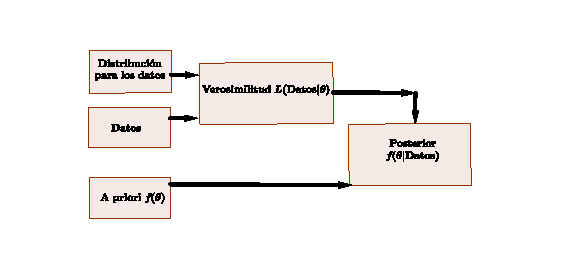
\includegraphics[scale=1.8]{bayes1.pdf}
\end{center}
\vspace{-2cm}\caption{\bf M\'etodo Bayesiano para realizar inferencia.}\label{eb}
\end{figure}
\noindent Las combinaciones de experiencias pasadas dan la informaci\'on a priori para formar un marco de referencia y tomar una decisi\'on que conlleve al mejoramiento de alg\'un proceso. En la mayor\'ia de las aplicaciones es necesario y \'util combinar informaci\'on a priori con datos experimentales. Por ejemplo,  supongamos que al realizar un estudio de confiabilidad los ingenieros expertos saben con cierta certeza, el tiempo promedio que tarda en fallar un componente.  
Adem\'as de  estudios anteriores, su tiempo de falla es Weibull con ciertos par\'ametros que se encuentra dentro de un rango espec\'ifico. Para estimar la distribuci\'on del ciclo de vida de un componente similar, este conocimiento previo puede ayudar a optimizar el  tama\~no de la muestra y a disminuir la incertidumbre  en la inferencia.


\noindent  A grandes rasgos el procedimiento para hacer inferencia Bayesiana sobre un vector de par\'ametros $\theta$, es el siguiente (Figura \ref{eb}):

\begin{itemize}
\item Conocimiento apriori acerca de $\theta$ expresado en t\'erminos de una funci\'on de densidad de probabilidad, denotada por $f(\theta)$.
\item La verosimilitud para los datos disponibles y un modelo especificado dado por $L(Datos|\theta)$.
\item Utilizar la regla de Bayes, para obtener una distribuci\'on posterior, que resulte de la combinaci\'on de la verosimilitud y el conocimiento de la distribuci\'on a priori de $\theta$. La distribuci\'on posterior es usada para cuantificar la incertidumbre de las cantidades de inter\'es.  
\end{itemize}
 

\noindent Uno de los primeros pasos para hacer estad\'istica Bayesiana consiste en obtener informaci\'on modelable en t\'erminos de una funci\'on de densidad.
La obtenci\'on de la distribuci\'on a priori para un solo par\'ametro puede ser sencilla, si se ha considerado la experiencia en situaciones similares. Para un vector de par\'ametros, establecer la distribuci\'on a priori conjunta puede ser mucho m\'as complicado. Tambi\'en es dif\'icil obtener informaci\'on sobre la dependencia de los par\'ametros y expresarlo en t\'erminos de una distribuci\'on conjunta. Por ejemplo, si la experiencia previa  de estimaciones pasadas para los par\'ametros de la distribuci\'on  lognormal $\mu$ y $\sigma$ indican que est\'an altamente correlacionados, significa que la distribuci\'on a priori para estos par\'ametros deber\'ia reflejar esta dependencia


\noindent Un enfoque adecuado para construir la distribuci\'on a priori, consiste en formular informaci\'on acerca de un cuantil en especial (o par\'ametros), de acuerdo a experiencia previa.\\[0.2cm]

\noindent  Al momento de elegir una distribuci\'on a priori, existen 3 tipos diferentes:
 \begin{itemize}
 \item Cuando se tiene la informaci\'on suficiente tales que los par\'ametros son conocidos, y conducen a una distribuci\'on degenerada\footnote{Una variable aleatoria $X$ es degenerada en un punto o conjunto $c\in \mathbb{R}$, si $P(X=x)=1$ si $x\in c$ y $P(X=x)=0$ si  $x\notin c.$}. 
 \item Informaci\'on difusa de los par\'ametros, que conduzcan una distribuc\'ion a priori no informativa.
 \item Una distribuci\'on a priori informativa no degenerada.
 \end{itemize}
 
 
\noindent Comunmente, las principales fuentes de informaci\'on para una distribuci\'on a priori son:
 
 \begin{enumerate}
 \item Opini\'on de expertos u otros.
 \item Informaci\'on de datos pasados.
 \end{enumerate}
 
\noindent  Finalmente podemos mencionar que el uso de una distribuci\'on a priori es un instrumento de modelaci\'on que permite descartar entornos o escenarios improbables. Este  instrumento de modelaci\'on  permite tomar una decisi\'on acerca de la forma que debe tener la funci\'on de distribuci\'on a priori.

\section{Inferencia Bayesiana}

\noindent Se puede observar que dadas dos variables aleatorias $X$, $Y$, la funci\'on de densidad $f(Y|X)$ es proporcional a $f(X,Y)$, en el siguiente sentido. Sabemos que
 $$f(y)=\int f(x,y)\,dx=\int f(x)f(y|x)\,dx,$$
 es claro que 
\begin{eqnarray}
f(y|x)=\frac{f(x,y)}{f(x)}=\frac{f(y)f(x|y)}{f(x)}.\label{pro}
\end{eqnarray}
Entonces $$f(Y|X)\propto f(Y)f(X|Y),$$
esta es una de las formas del teorema de Bayes y es la utilizada dentro de la estad\'istica Bayesiana. La igualdad esta bien definida para variables discretas y continuas  {\bf  [\ref{PL}]}. La constante
 de proporcionalidad, es el denominador de la expresi\'on (\ref{pro}), y es necesaria para que $f(Y|X)$ sea una distribuci\'on de probabilidad. En el caso continuo se determina por

$$\frac{1}{f(x)}=\frac{1}{\int f(x,y)\,dy},$$y en el caso discreto es 
$$\frac{1}{f(x)}=\frac{1}{\sum_{y} f(x,y)}.$$



\noindent Veamos un ejemplo artificial de la manera en la cu\'al se aplica el teorema de Bayes.

\subsubsection{Ejemplo}
\noindent Supongamos que $Y$ es la variable aleatoria que describe el tiempo en que falla por primera vez cierto objeto {\bf  [\ref{PL}]}, el cual es medido por un instrumento que tiene un peque\~no retraso en  la medici\'on. Sea $X$ el tiempo de registro del instrumento, es decir, X es mayor que Y, pero solo es posible observar $X$ y necesitamos concluir algo acerca de $Y$. Supongamos adem\'as que se sabe que
\begin{eqnarray*}
f(y)&=&\exp\{-y\} \mbox{  } (0<y<\infty)\\
f(x|y)&=&k\exp\{-k(x-y)\}  \mbox{  } (y<x<\infty)
\end{eqnarray*}

\noindent Entonces para hacer conclusiones del comportamiento de $Y$ dado $X$, necesitamos a  $f(Y|X)$. Aplicando el teorema de Bayes citado anteriormente se tiene que
\begin{eqnarray*}
f(y|x) &\propto& f(y)f(x|y)\\
&\propto& k\exp\{-y\}\exp\{-k(x-y)\} \\
&\propto& \exp\{(k-1)y\}  \mbox{  } (0<y<x).
\end{eqnarray*}

\noindent Con frecuencia es suficiente con obtener este resultado, pero la constante de proporcionalidad es necesaria para que lo que se esta obteniendo sea un distribuci\'on de probabilidad, en este caso la constante de proporcionalidad es:

\begin{eqnarray*}
\int_{0}^{x}  \exp\{(k-1)y\}dy &=& \frac{1}{k-1}\left[\exp\{(k-1)x\}-1\right].
\end{eqnarray*}
\newpage

\noindent Si estamos interesados en $k$ par\'ametros desconocidos $$\theta=(\theta_1,\theta_2,\cdots,\theta_k)$$ y tenemos la creencia de alguna distribuci\'on a priori para estos valores expresada en t\'erminos de la distribuci\'on de probabilidad $f(\theta)$, contamos con $n$ observaciones de una muestra del experimento a observar $$X=(x_1,x_2,\cdots,x_n)$$
con una distribuci\'on de probabilidad que depende de estos $k$ par\'ametros desconocidos. Entonces los componentes de $X$ son variables aleatorias y la dependencia de $X$ sobre $\theta$,  puede ser expresada en t\'erminos de una funci\'on de densidad de probabilidad (fdp) $$f(X|\theta).$$

\noindent Es posible encontrar una manera de expresar la distribuci\'on de inter\'es considerando la distribuci\'on a priori y los datos. La herramienta b\'asica es el teorema de Bayes para variables aleatorias, este afirma que

$$f(\theta|X)\propto f(\theta)f(X|\theta),$$
la funci\'on $f(X|\theta)$, como funci\'on de $X$ y fijando $\theta$ es una densidad, sin embargo $f(X|\theta)$ como funci\'on de $\theta$ la llamamos funci\'on de verosimilitud y con frecuencia la escribimos como $$L(\theta|X)=f(X|\theta).$$

\noindent Con $f(\theta)$ como la distribuci\'on a priori para $\theta$ y $f(\theta|X)$ como la distribuci\'on posterior para $\theta$ dado $X$, el teorema de Bayes se transforma en su forma m\'as memorable:
 
\begin{center}
\begin{tabular}{|c|}
\hline
Posterior $\propto$ A priori $\times$ Verosimilitud.\\
\hline
\end{tabular}
\end{center}


\noindent La relaci\'on anterior resume, el camino en el cual deber\'iamos modificar nuestra creencia considerando los datos disponibles. Para una muestra inicial de $X$ observaciones 
\begin{eqnarray}
f(\theta|X)\propto f(\theta)L(\theta|X).\label{poscita}
\end{eqnarray}
\noindent Los c\'alculos y conclusiones anteriores se sintetizan en el siguiente teorema.
\begin{thm}
La distribuci\'on posterior $f(\theta|X)$ es la distribuci\'on condicional de $\theta$ dado los datos, expresada por:

\begin{eqnarray*}
f(\theta|X)&=&\frac{L(X|\theta)f(\theta)}{\int_{\Omega} L(X|\theta)f(\theta)\,d\theta},
\end{eqnarray*}
donde $\Omega$ es el espacio param\'etrico de $\theta$ y $f(\theta)$ es la distribuci\'on a priori para  $\theta$.\\[0.2cm]
De aqu\'i:
$$f(\theta|X)\propto L(X|\theta)f(\theta)$$
y
$$f(X)=\int L(X|\theta)f(\theta)\,d\theta,$$
a esta \'ultima expresi\'on se le suele llamar verosimilitud integrada. Es en realidad la distribuci\'on marginal de los datos, vista como funci\'on de $X$.
\end{thm}

\noindent La distribuci\'on posterior es  una distribuci\'on para los par\'ametros de la distribuci\'on y en la mayor\'ia de las veces es de inter\'es hacer inferencia sobre alguna observaci\'on $X$, y no sobre los par\'ametros. Para realizar esta inferencia se emplea la distribuci\'on predictiva.

 \begin{thm}
 Bajo el supuesto de que existe independencia entre los datos $X$, dados los par\'ametros $\theta$, para la observaci\'on futura $y$, la distribuci\'on predictiva posterior es:
 $$f(y|X)=\int_{\theta} f(y|\theta)f(\theta|X) d\theta=E_{(\theta|X)}[f(y|\theta)],$$
 \end{thm}

\noindent La demostraci\'on del teorema anterior se puede ver en Bernando y Smith(1994). [{\bf \ref{BT}}]\\[0.1cm]
\noindent El ejemplo siguiente ilustra la forma de realizar inferencia sobre los par\'ametros de una distribuci\'on.

\subsubsection{Ejemplo}
\noindent Supongamos que lanzamos de una moneda  no justa y observamos el resultado. Modelamos el experimento con variables aleatorias Bernoulli de par\'ametro $p$, $x_i\sim$Ber ($p$). Dado que es una moneda no justa, tenemos conocimiento a priori de $p$, modelada como una variable aleatoria Beta, $p\sim$Beta$(\alpha, \beta)$. Para deducir conclusiones acerca de este experimento necesitamos hallar la distribuci\'on posterior de $p$ dado los datos, utilizando la expresi\'on (\ref{poscita}).\\


\noindent La verosimilitud esta dada por
\begin{eqnarray} \label{vee}
f(X|p)= p^{\sum x_i}(1-p)^{n-\sum x_i}.
\end{eqnarray}
La distribuci\'on a priori de $p$ es: 
\begin{eqnarray} \label{ap}
f(p)=\frac{\Gamma(\alpha)\Gamma(\beta)}{\Gamma(\alpha + \beta)} p^{\alpha-1}(1-p)^{\beta-1}\mbox{I}_{[0,1]}(p)
\end{eqnarray}

La distribuci\'on posterior usando (\ref{vee}),  (\ref{ap}) y sustituyendolas en (\ref{poscita}) es
\begin{eqnarray*} 
f(p|X)&\propto& f(X|p)f(p)\\
&\propto& p^{\sum x_i +\alpha-1}(1-p) \mbox{I}_{[0,1]}(p),
\end{eqnarray*}
esta \'ultima expresi\'on puede ser completada para que sea una distribuci\'on Beta, por lo tanto 

$$p|X\sim \mbox{Beta} (\alpha + \sum x_i, \beta+n-\sum x_i).$$

\noindent La distribuci\'on posterior encontrada pertenece a la misma familia que la distribuci\'on a priori. Cuando se tienen casos como los anteriores en donde la distribuci\'on a priori y la posterior se distribuyen de la misma manera pero con diferentes par\'ametros son llamadas distribuciones conjugadas.


%
%\subsection{Distribuci\'on predictiva}
%
%En muchas de las aplicaciones necesitamos calcular  la distribuci\'on marginal 
%$$p(X)=\int p(X|\theta)p(\theta)\,d\theta$$
%la cual es llamada distribuci\'on predictiva de $X$.

%Cualquier informaci\'on emp\'irica, combinada con el conocimiento que ya se tenga del problema que se estudia y actualiza dicho conocimiento.

%
%\subsection{Familias conjugadas}
%
%Tanto $p(\theta)$ como $p(\theta|x)$ son distribuciones de probabilidad sobre $\theta$: como sabemos la primera incorpora informaci\'on a priori y la segunda actualiza dicha informaci\'on muestral que se puede obtener. Si bien dijimos que la elecci\'on de una u otra distribuci\'on de probabilidad  para modelar nuestra incertidumbre sobre $\theta$ no resulta crucial en tanto sea factible e licitar con cualquiera de ellas una distribuci\'on a priori, resulta conveniente que $p(\theta)$ y $p(\theta|x)$ pertenezcan a la misma familia.
%\\[0.3cm]
%
%Definici\'on: Sea $P:=\{p(x|\theta): \theta \in \Omega\}$ una familia param\'etrica. Una clase (o colecci\'on) de distribuciones de probabilidad $F$ es una familia conjugada para $P$ si para todo $p(x|\theta)\in P$ y $p(\theta)\in F$ se cumple que $p(\theta|x)\in F$.\\[0.2cm]
%
%Uno de los principales objetivos de la teor\'ia de decisi\'on en el desarrollo de procesos l\'ogicos para la toma de decisiones bajo condiciones de incertidumbre. La idea es plantear los problemas  de inferencia estad\'istica como problemas de decisi\'on y aprovechar por tanto los resultados que ya se tienes respecto a esto ultimo.
%\\[0.2cm]
%Al momento de resolver un problema de decisi\'on existen diversas formar que nos interesa para hacer inferencia desde el enfoque bayesiano y para ello requerimos tener identificado lo siguiente:
%
%\begin{itemize}
%\item El espacio de estados $\Omega$.
%\item Una funci\'on de probabilidad $P$ sobre los elementos de $\Omega$,
%\item Una funci\'on de utilidad $u$ sobre $C$.
%\end{itemize}
%
%


\subsection{M\'etodo de Simulaci\'on}
\noindent Antes de la aparici\'on de m\'etodos computacionales las distribuciones conjugadas eran las empleadas en estad\'istica Bayesiana, por la facilidad de los c\'alculos. Sin embargo limitaba en gran medida el manejo de las distribuciones a priori y de los posibles modelos. Actualmente los procedimientos computacionales han realzado el empleo de este enfoque estad\'istico, puesto que se puede proponer la distribuci\'on a priori adecuada, sin forzarla a que sea necesariamente conjugada, permitiendo que al momento de obtener la distribuci\'on posterior, aunque se tenga una expresi\'on bastante compleja,  puedan obtenerse  aproximaciones de esta distribuci\'on. Estas aproximaciones se ven reflejadas en la simulaci\'on de datos de la distribuci\'on posterior. A finales de los a\~nos 80's surgieron m\'etodos de simulaci\'on para realizar c\'alculos de este tipo, uno de los m\'as utilizados son los algoritmos Markov Chains Monte Carlo (MCMC).\\[0.1cm]
\noindent El algoritmo MCMC (Markov Chain Monte Carlo) es una clase general de algoritmos usados para producir muestras de la distribuci\'on posterior, en altas dimensiones. El objetivo b\'asico de un algoritmo MCMC es simular valores o muestras de una distribuci\'on posterior  de un vector de par\'ametros. Tiene la propiedad de que la distribuci\'on de la $j$-\'esima iteraci\'on en la secuencia de valores muestrales, convergen a una muestra aleatoria de la distribuci\'on posterior para $j$ grande. En general muestras sucesivas de la distribuci\'on posterior est\'an correlacionadas, pero esta correlaci\'on tiende a perderse conforme el tama\~no de la muestra crece. As\'i para valores grandes de la muestra se actualizan los \'ultimos grupos dentro de una secuencia, digamos $\theta^{(m)}$, $\theta^{(m+1)} \cdots \theta^{(m+k)}$ y estos representan la muestra de la distribuci\'on posterior de inter\'es.\\[0.1cm]
\noindent Consideremos dos tipos de algoritmos MCMC: Metropolis- Hasting y Gibbs samplers. A continuaci\'on mencionaremos las ideas b\'asicas de estos algoritmos.

\subsubsection{ Muestreo Gibbs.}
\noindent El muestreo Gibbs  es probablemente uno de los algoritmos MCMC m\'as usados dentro de la estad\'istica Bayesiana [{\bf \ref{mi}}]. El t\'ermino formal fue establecido por  Geman y Geman[{\bf \ref{geman}}], cuando estudiaban modelos de procesamiento de im\'agenes. El muestreo Gibbs es un m\'etodo para generar datos de variables aleatorias sin tener que realizar expl\'icitamente los c\'alculos que se  involucran para obtener la densidad, se basa en propiedades de las cadenas de Markov.
Cassella y George(1992) dan una tutorial acerca de este m\'etodo [{\bf \ref{gibbs}}].\\[0.12cm]
\noindent  A grandes rasgos un Muestreo Gibbs se construye de la siguiente manera.\\[0.1cm]
\noindent Supongamos que tenemos un vector de par\'ametros 
$\theta=(\theta_1,\cdots,\theta_q)$ y denotamos las distribuciones posteriores condicionales totales (full conditionals) por :\\
$f_1(\theta_1|\theta_2,\cdots,\theta_q,datos)$, 
$f_2(\theta_2|\theta_1,\theta_3\cdots,\theta_q,datos)$, 
$\cdots $, $f_q(\theta_q|\theta_1,\cdots,\theta_{q-1},datos)$.


\begin{description}
\item[PASO I:] Generar un valor inicial $\theta^{0}=(\theta_1^{0},\cdots,\theta_p^{0})$ y considerar j=0.

\item[PASO II:]
Construir $\theta^{j+1}=(\theta_1^{j+1},\cdots,\theta_p^{j+1})$ de la siguiente manera:
\begin{itemize}
 \item Generar $\theta_1^{j+1} \sim f_1(\theta_1|\theta_2,\cdots,\theta_q,datos)$;
 \item Generar $\theta_2^{j+1}\sim f_2(\theta_2|\theta_1,\cdots,\theta_q,datos)$ $\cdots$
 \item Generar $\theta_{q}^{(j+1)}\sim f_q(\theta_q|\theta_1,\cdots,\theta_{q-1},datos).$ 
\end{itemize}
\item[PASO III:] incrementar $j$ y regresar al paso II.
\item[PASO IV:] Regresar $\{\theta^{(1)},\theta^{(2)}\cdots \theta^{(M)}\}$
\end{description}

\noindent Gelfand y Smith (1992) mostraron que bajo ciertas condiciones de regularidad, el vector generado  tiene distribuci\'on estacionaria $f(\theta|Datos)$ utilizando ciertas propiedades de cadenas de Markov.

\subsubsection{Metropolis Hastings}
\noindent Las primeras ideas del algoritmo Metropolis-Hastigs fueron introducidas en el art\'iculo
``The Monte Carlo Method'' por Metropolis and Ulam(1949), mostrando un ejemplo de estimaci\'on de probabilidades de \'exito para una estrategia del solitario, realizando muchos intentos y   calculando la proporci\'on de \'exito. El m\'etodo fue generalizado y probado m\'as tarde por el profesor de la universidad de Toronto  llamado W. Keith Hasting(1970). David B. Hitchcock(2003) proporciona una historia detallada sobre el nacimiento de este m\'etodo. {\bf [\ref{MH}}]

\noindent Metropolis Hasting es un algoritmo de simulaci\'on al igual que Muestro Gibbs, solo que un poco m\'as general. Su mayor peso recae en la selecci\'on de una distribuci\'on propuesta.
\noindent Supongamos que $\pi(x)$ es la distribuci\'on objetivo, por ejemplo, es la distribuci\'on posterior, de la que se desea simular. La distribuci\'on ``propuesta'' es una distribuci\'on condicional $q(y|x)$ y constituye ``una sugerencia'' de pasar de un estado $x$ a  un punto $y$. [{\bf \ref{UMH}}]\\
\noindent De manera general el algoritmo es el siguiente [{\bf \ref{mi}}]: 

\begin{description}
\item[{\bf  PASO I:}] Iniciar con un valor $x^{(t)}$  dentro del soporte de la distribuci\'on objetivo.

\item[{\bf PASO II:}] Generar un valor candidato $y^{(t)}\sim q(\cdot|x^{(t)})$.

\item [{\bf PASO III:}] Generar $u_t \sim $Uniforme$(0,1)$ si 

$$u < \min \left\{\frac{\pi(y)}{\pi(x)}\frac{q(x|y)}{q(y|x)},1\right\},$$  
hacer $x^{(t+1)}=y^{(t)}$, si no rechazar y hacer $x^{(t+1)}=x^{(t)}$.
\item  [{\bf PASO IV:}]Regresar al paso II.
\item [{\bf PASO V:}] Regresar $\{x^{t},x^{t+1},\cdots, x^{t+M}\}$.
\end{description}
\noindent El \'exito del algoritmo depende de la selecci\'on de la distribuci\'on propuesta. Como lo discutido por Chib and Greenberg, [{\bf \ref{UMH}}] la propagaci\'on de la densidad propuesta afecta el comportamiento de la cadena de Markov en dos sentidos:
una es el rango de aceptaci\'on (el porcentaje de veces que se mueve de un punto a otro ) y la otra es la regi\'on del espacio donde se mueve la cadena. Para construirla se deben considerar ciertas propiedades [{\bf \ref{UMH}}].\\[0.1cm]
\noindent Los m\'etodos anteriores  se emplean para producir datos de la distribuci\'on posterior y realizar estimaciones sobre estos.


\subsection{Estimaci\'on  Bayesiana}
\noindent Una vez generada la muestra de la distribuci\'on posterior es de inter\'es obtener estimadores basados en la muestra obtenida, realizar inferencia y pron\'osticos de funciones que revelen el comportamiento del fen\'omeno modelado. A continuaci\'on mencionaremos la manera de realizar estas estimaciones utilizando la muestra de la distribuci\'on posterior.\\


\noindent Una estimaci\'on com\'un despu\'es de obtener la muestra,  es encontrar la media posterior para alguna funci\'on $g(\theta)$.
\noindent Si $f(\theta|Datos)$ es la densidad de probabilidad posterior, entonces la media se obtiene como:
\begin{eqnarray}\label{a}
E[g(\theta)|Datos]=\int g(\theta)f(\theta|Datos)\,d\theta.
\end{eqnarray}
Por otro lado, si suponemos que la muestra  de la distribuci\'on posterior es $\theta_1^{*},\theta_2^{*},\cdots,\theta_M^{*}$, entonces por la ley de los grande n\'umeros, la media posterior de $g(\theta)$ se aproxima por
\begin{eqnarray*}\
\hat{g}(\theta)\approx\frac{1}{M^{*}}\sum_{i=1}^{M^{*}}g(\theta_i^{*}).
\end{eqnarray*}
\noindent Los m\'etodos Bayesianos son tambi\'en usados para predecir un evento futuro. Las fallas de un determinado componente en un proceso espec\'ifico, pueden predecirse usando la distribuci\'on posterior predictiva. Una manera de calcularla es utilizando la muestra de la distribuci\'on posterior, es a trav\'es de un promedio. De la siguiente manera:
\begin{eqnarray}\label{c}
f (x|Datos)\approx \frac{1}{M^*}\sum_{i=1}^{M^*}f(x|\theta_i^*),
\end{eqnarray}
\noindent para cada $x$ dentro del dominio de la distribuci\'on posterior.\\[0.1cm]

\noindent Similarmente la cdf posterior predictiva es aproximada por el valor esperado de la cdf posterior 
\begin{eqnarray}\label{b}
F(x|Datos)\approx \frac{1}{M^*}\sum_{i=1}^{M^*}F(x|\theta_i^*),
\end{eqnarray}
\noindent para cada $x$ dentro del dominio de la distribuci\'on posterior.\\[0.1cm]



\noindent Una vez que se tenga la muestra de la distribuci\'on posterior, podemos calcular todas las funci\'ones que caractericen al fen\'omeno modelado, tales como la funci\'on de confiabilidad y la de riesgo, que ser\'an de inter\'es en los cap\'itulos posteriores.
\newpage \thispagestyle{empty} \cleardoublepage


\chapter{Transformadores y Estad\'istica Bayesiana}

\noindent En esta tesina se propone un plan de inventario de transformadores de instrumento,
 desde un enfoque Bayesiano. Para lograr esta meta, se necesita primero conocer aspectos exploratorios sobre el comportamiento del tiempo de  vida de los transformadores.  
 
 
\noindent Para empezar el estudio que nos conduzca al plan de inventario o almacenamiento, tenemos que realizar inferencia 
sobre los datos e informaci\'on disponible.\\[0.1cm] 
En este cap\'itulo se hace el an\'alisis de los datos,  proponiendo 
una distribuci\'on a priori, para combinarla con la funci\'on de verosimilitud y tener la distribuci\'on 
posterior, para conseguir conclusiones acerca del comportamiento de los tiempos de vida de
los transformadores.


\begin{table}[h!]\small
\begin{center}
\caption {\bf Tiempos de vida de transformadores de corriente, $t_i$ (meses), $e_i=1$ indica un dato censurado, $e_i=0$ es un dato no censurado.\label{uno}}
\begin{tabular}{ccc|ccc|ccc|ccc}
\toprule[0.6mm]
$i$	&	$t_i$	&	$t_i$	&	$i$	&	$t_i$	&$e_i$	&	$i$	&	$t_i$	&	$e_i$	&	$i$	&	$t_i$	&	$e_i$	\\
\toprule[0.6mm]
1	&	8	&	1	&	36	&	107	&	0	&	106	&	272	&	1	&	141	&	308	&	0	\\
2	&	8	&	1	&	37	&	116	&	1	&	107	&	272	&	1	&	142	&	308	&	0	\\
3	&	8	&	1	&	38	&	119	&	0	&	108	&	272	&	1	&	143	&	308	&	1	\\
4	&	8	&	1	&	39	&	119	&	0	&	109	&	272	&	1	&	144	&	308	&	1	\\
5	&	8	&	1	&	40	&	139	&	0	&	110	&	272	&	1	&	145	&	308	&	1	\\
6	&	20	&	1	&	41	&	140	&	0	&	111	&	274	&	0	&	146	&	308	&	1	\\
7	&	20	&	1	&	42	&	144	&	0	&	112	&	274	&	0	&	147	&	308	&	1	\\
8	&	20	&	1	&	43	&	146	&	0	&	113	&	274	&	0	&	148	&	308	&	1	\\
9	&	20	&	1	&	44	&	146	&	0	&	114	&	275	&	0	&	149	&	308	&	1	\\
10	&	32	&	1	&	45	&	152	&	1	&	115	&	275	&	0	&	150	&	308	&	1	\\
11	&	32	&	1	&	46	&	159	&	0	&	116	&	275	&	0	&	151	&	308	&	1	\\
12	&	32	&	1	&	47	&	159	&	0	&	117	&	276	&	0	&	152	&	308	&	1	\\
13	&	32	&	1	&	48	&	159	&	0	&	118	&	281	&	0	&	153	&	308	&	1	\\
14	&	32	&	1	&	49	&	160	&	0	&	119	&	281	&	0	&	154	&	308	&	1	\\
15	&	32	&	1	&	50	&	161	&	0	&	120	&	284	&	0	&	155	&	308	&	1	\\
16	&	32	&	1	&	51	&	164	&	1	&	121	&	284	&	0	&	156	&	308	&	1	\\
17	&	56	&	1	&	52	&	167	&	0	&	122	&	284	&	0	&	157	&	308	&	1	\\
18	&	80	&	1	&	53	&	172	&	0	&	123	&	284	&	0	&	158	&	308	&	1	\\
19	&	80	&	1	&	54	&	172	&	0	&	124	&	286	&	0	&	159	&	308	&	1	\\
20	&	80	&	1	&	55	&	176	&	1	&	125	&	286	&	0	&	160	&	308	&	1	\\
21	&	80	&	1	&	56	&	183	&	0	&	126	&	286	&	0	&	161	&	308	&	1	\\
22	&	80	&	1	&	57	&	188	&	1	&	127	&	287	&	0	&	162	&	308	&	1	\\
23	&	80	&	1	&	58	&	203	&	0	&	128	&	288	&	0	&	163	&	308	&	1	\\
24	&	80	&	1	&	59	&	205	&	0	&	129	&	288	&	0	&	164	&	308	&	1	\\
25	&	80	&	1	&	60	&	214	&	0	&	130	&	288	&	0	&	165	&	308	&	1	\\
26	&	80	&	1	&	61	&	214	&	0	&	131	&	288	&	0	&	166	&	308	&	1	\\
27	&	80	&	1	&	62	&	215	&	0	&	132	&	296	&	1	&	167	&	308	&	1	\\
28	&	80	&	1	&	63	&	216	&	0	&	133	&	296	&	1	&	168	&	308	&	1	\\
29	&	80	&	1	&	64	&	216	&	0	&	134	&	296	&	1	&	169	&	308	&	1	\\
30	&	80	&	1	&	65	&	216	&	0	&	135	&	296	&	1	&	170	&	308	&	1	\\
31	&	80	&	1	&	66	&	218	&	0	&	136	&	298	&	0	&	171	&	308	&	1	\\
32	&	80	&	1	&	67	&	218	&	0	&	137	&	299	&	0	&	172	&	308	&	1	\\
33	&	94	&	0	&	68	&	218	&	0	&	138	&	300	&	0	&	173	&	308	&	1	\\
34	&	94	&	0	&	69	&	225	&	0	&	139	&	308	&	0	&		&		&		\\
35	&	94	&	0	&	70	&	225	&	0	&	140	&	308	&	0	&		&		&		\\
\bottomrule[0.6mm]
\end{tabular}
\end{center}
\end{table}


\section{Distribuci\'on Apriori}
\noindent Los elementos disponibles dentro del estudio, 
es una base de datos de transformadores de instrumento de corriente en las sub\'areas de  
Coatzacoalcos y Temascal. Se disponen de sus tiempos de vida  a lo largo de 26 a\~nos hasta el 2006, con datos censurados y no 
censurados. 

\noindent Los datos se muestran en la Tabla \ref{uno}, representados de la siguiente manera, 
$(\underline{t},\underline{e})=\{t_i,e_i\}^n_{i=1}$, donde $e_i=1$ indica que 
el transformador $i$ aun sigui\'o en 
operaci\'on al final de 2006, lo que implica que  es un dato censurado por la derecha. Mientras que $e_i=0$, se refiere a un valor no censurado. De estudios 
anteriores realizados por el CIMAT, los tiempos de vida son modelados adecuadamente 
por medio de una 
distribuci\'on Weibull. La funci\'on de Verosimilitud bajo 
este modelo se expresa 
de la siguiente manera:
\begin{eqnarray}\label{tiempos}
f(\underline{t}|\underline{e},\beta,\eta)&=& \prod_{e_i=0}\frac{\beta}{\eta}\left(\frac{t_i}{\eta}\right)^{\beta-1}\exp \left\{-\left(\frac{t_i}{\eta}\right)^{\beta}\right\}\prod_{e_i=1}\exp\left\{-\left(\frac{t_i}{\eta}\right)^{\beta}\right\}.
\end{eqnarray}

\noindent Para iniciar la inferencia de los datos disponibles, necesitamos proponer una distribuci\'on a priori que refleje el conocimiento que se tiene acerca del fen\'omeno a modelar. Elegimos como modelo para los par\'ametros  $\beta$ y $\eta$ distribuciones gammas, con la siguiente notaci\'on:
\begin{eqnarray}\label{beta}
\beta\sim Ga(a_1,b_1)
\end{eqnarray}
 y 
  \begin{eqnarray}\label{eta}
 \eta\sim Ga(a_2,b_2). 
 \end{eqnarray}
 
\noindent La raz\'on por la cual elegir  distribuciones Gammas para las a  prioris  es su flexibilidad, pueden obtenerse formas sesgadas a la derecha, izquierda o centradas. Cabe mencionar que la elecci\'on de una distribuci\'on a priori  espec\'ifica, solo se debe de interpretar como un medio o instrumento  que nos ayudar\'a a modelar la informaci\'on disponible.\\[0.2cm]
 \noindent Una vez elegidos los instrumentos de modelaci\'on, es de inter\'es establecer los par\'ametros para las a prioris, estos se fijar\'an con la ayuda de dos elementos:
\begin{itemize}
\item  La distribuci\'on predictiva a priori.
\item  El comportamiento de la funci\'on de riesgo de los transformadores.
\end{itemize}

\begin{figure}
\begin{center}
\includegraphics[scale=0.4]{r1.png}
\end{center}
\vspace{-1 cm}\caption{\bf Posibles funciones de riesgo para la distribuci\'on predictiva a priori.}\label{trestt}
\end{figure}


\noindent Primero hablaremos acerca de la funci\'on de riesgo.  Esta funci\'on describe el desgaste de los transformadores a lo largo del tiempo. Al empezar su funcionamiento, el riesgo a fallar es peque\~no y conforme pasa el tiempo, debido al uso, el ambiente y otros factores, el riesgo aumenta paulatinamente. La determinaci\'on o modelaci\'on de las distribuciones a priori tienen como misi\'on descartar entornos improbables de los fen\'omenos que modelan. En la Figura  \ref{trestt} se observan tres trayectorias posibles de riesgo.
Si la vida de los transformadores tiene una funci\'on de riesgo decreciente, indica  que al momento de iniciar su vida \'util, el riesgo a fallar es alto y conforme pasa el tiempo, se reduce.  Sin embargo existen factores como la humedad que no permiten que el riesgo de falla de un transformador disminuya, sino al contrario.\\[0.1cm]
\noindent  Por otra parte si la funci\'on de riesgo es constante, se concluir\'ia que los transformadores no se degradan a trav\'es del tiempo. Lo que no ocurre dadas las condiciones de uso.
\noindent As\'i la funci\'on de riesgo adecuada, es aquella que indique que en los primeros a\~nos de vida su riesgo es peque\~no y a lo largo del tiempo este riesgo aumenta. Una funci\'on de riesgo creciente es la m\'as razonable de acuerdo al funcionamiento de los transformadores. 

\noindent Por lo tanto la distribuci\'on a priori propuesta debe tener una funci\'on de riesgo creciente, esto es el par\'ametro $\beta$ tiene que ser mayor que $1$. \\[0.1cm]
\noindent
El siguiente paso, es observar el comportamiento de la distribuci\'on predictiva a priori. Previamente se mencion\'o la manera en la cual se obtiene la distribuci\'on predictiva posterior, sin embargo no se coment\'o nada al respecto de la {\bf distribuci\'on predictiva a priori}.  Al momento de asignar una distribuci\'on de probabilidad a los par\'ametros ($\beta$, $\eta$), estos no tienen interpretaci\'on cuantificable por experiencias. No es posible conocer expl\'icitamente sus valores por observaciones previas, solo tenemos conocimiento del fen\'omeno en general. Si se sabe la manera a priori del comportamiento del tiempo de vida de los transformadores entonces se tiene conocimiento de la distribuci\'on predictiva a priori. Esta distribuci\'on esta dada por:

 $$f(t)=\int_{\beta,\eta}f(t|\beta,\eta)  f(\beta,\eta)d\beta d \eta,$$
 
 \noindent donde  $f(\beta,\eta)$ es la distribuci\'on conjunta a priori de $\beta$ y $\eta$.
\noindent Por experiencia podemos conocer ciertas caracter\'isticas del tiempo de vida de los transformadores y  tener informaci\'on previa de  $f(t)$. Esta informaci\'on determina un rango de valores para $\beta$ y $\eta$. La manera m\'as com\'un de establecer la distribuci\'on  a priori predictiva es empleando dos cuantiles. Como describiremos en los siguientes p\'arrafos.\\[0.1cm]


%\\[0.2cm]
\begin{figure}
\begin{center}
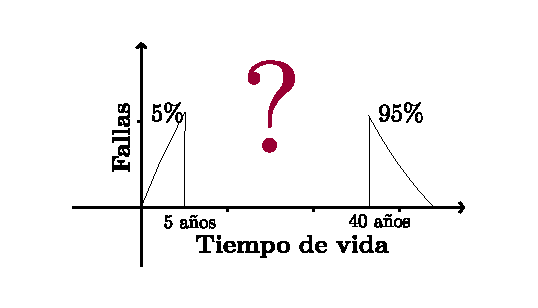
\includegraphics[scale=1]{apriori1.pdf}
\end{center}
\vspace{-1.5 cm}\caption{\bf Distribuci\'on predictiva a priori a modelar.}\label{dos}
\end{figure}

\noindent  Suponiendo que el $5\%$ de los transformadores fallan en los primeros 5 a\~nos (80 meses) y  que el $95\%$ de ellos ya fallaron a los $40$ a\~nos (480 meses) o antes, y 
si adem\'as $$T\sim \text{Weibull}(\eta^{*},\beta^{*})$$ 


\noindent es la variable aleatoria a priori que modela el tiempo de vida de los transformadores. La Figura \ref{dos} muestra la distribuci\'on a priori predictiva, con los cuantiles fijados en los extremos. Sin embargo el centro de la distribuci\'on debe ser modelada.\\[0.1cm]
\noindent La informaci\'on de los cuantiles se representa por:
$$P(T\leq 80)=0.05$$
y 
$$P(T\leq 480)=0.95.$$

\noindent Con esta informaci\'on es posible conocer  $\eta^{*}$ y  $\beta^{*}$  de la siguiente forma, se sabe que para una variable aleatoria Weibull
\begin{eqnarray*}
P(T\leq t) &=& 1-\exp\left\{-\left(\frac{t}{\eta}\right)^{\beta}\right\}
\end{eqnarray*}

Por lo tanto debemos resolver
\begin{eqnarray*}
0.05 &=& 1-\exp\left\{-\left(\frac{t}{\eta^{*}}\right)^{\beta^{*}}\right\}\\
0.95 &=& 1-\exp\left\{-\left(\frac{t}{\eta^{*}}\right)^{\beta^{*}}\right\}\\
\end{eqnarray*}

Resolviendo el sistema se llega a que

\begin{eqnarray*}
\beta^{*}&=& 1.955\\
\eta^{*}&=& 273.8
\end{eqnarray*}

\noindent Los par\'ametros encontrados describen el comportamiento a priori del tiempo de vida, no de los par\'ametros $\beta$  y $\eta$. Con ayuda de estos datos se pueden obtener los par\'ametros $a_1, b_1, a_2$ y $b_2$, que como lo mencionamos al inicio de la secci\'on son los par\'ametros, para las distribuciones Gammas de  $\beta$ y $\eta$ respectivamente, notando lo siguiente:

\begin{enumerate}
\item[{\bf 1.-} ]
\noindent  Como $\beta^{*}= 1.955$, quiere decir que los valores que produzca la distribuci\'on Gamma con par\'ametros $a_1$ y $b_1$ oscilaran alrededor de estos valores. Similarmente como $\eta^{*}= 273.8$ significa que los valores que tome la distribuci\'on $Ga(a_2,b_2)$ estar\'an alrededor de 273.8 aproximadamente.
\item[{\bf 2.-} ]
\noindent De manera general  la funci\'on de densidad de una variable aleatoria Gamma con par\'ametros $a$ y $s$, representada como $Ga(a,s)$ es

$$f(x)=\frac{1}{s^a\Gamma(a)}x^{a-1}\exp\left\{\frac{x}{s}\right\}$$
y su valor esperado esta dado por:
\begin{eqnarray*}
E(X)&=& as.
\end{eqnarray*}

\noindent Del hecho de que  $\beta\sim $Gamma$(a_1,b_1)$ y  juntando las dos aseveraciones anteriores se tiene que: 
$\beta^{*}=1.955\approx E(\beta)=a_1b_1$, as\'i $$b_1=\frac{1.955}{a_1}.$$


De manera similar para  $\eta\sim $Gamma$(a_2,b_2)$ se obtiene

$\eta^{*}=273.8\approx E(\eta)=a_2b_2$, de donde
 $$b_2=\frac{273.8}{a_2}.$$

\end{enumerate}
Tanto $b_1$ como $b_2$ quedan expresadas en funci\'on de $a_1$ y $a_2$, que son los par\'ametros de forma para $\beta$ y $\eta$ respectivamente.\\[0.1cm]
Para  fijar $a_1$ y $a_2$, se  proponen distintos valores para estos par\'ametros. Para cada uno de los valores propuestos se obtienen sus respectivas $b_1$ y $b_2$, con lo que queda de manera expl\'icita establecidas las distribuciones a priori. Una vez teniendo estas a prioris se produce la distribuci\'on predictiva a priori y la funci\'on de riesgo. Luego se eval\'ua que tan cerca se encuentra la a priori predictiva de la informaci\'on que se esta modelando, para finalmente elegir $a_1$ y $a_2$ que ajusten  de manera razonable la informaci\'on a priori.

\noindent Realizando el procedimiento anterior se fijaron los siguiente valores
$a_1=25$,  $b_1 =0.092$, $a_2=12$ y  $b_2 =2.2$. La Figura \ref{risk1} muestra la densidad predictiva a priori  con los valores establecidos, y la Figura \ref{risk2} muestra la funci\'on de riesgo, se ha modelado de manera creciente. 

\begin{figure}
\centering
\includegraphics[scale=0.2]{app.pdf}
\vspace{-0.5cm}\caption{{\bf Funci\'on de densidad a priori.}\label{risk1}}
\end{figure}


\begin{figure}
\centering
\includegraphics[scale=0.2]{r2meses.pdf}
\vspace{-0.5cm}\caption{{\bf Funci\'on de riesgo a priori.}\label{risk2}}
\end{figure}

\section{Distribuci\'on  Posterior}
\noindent Recordando que  $T$ es la variable aleatoria que representa los tiempo de vida de los transformadores, su funci\'on de verosimilitud esta dada por (\ref{tiempos}) y las distribuciones (\ref{beta}), (\ref{eta}). 
La distribuci\'on posterior es 

\begin{eqnarray*}
f(\beta,\eta|T)&\propto&\mbox{Verosimilitud} \times \mbox{A priori} \\
&=& f(T|\beta,\eta)f(\beta,\eta)
\end{eqnarray*}
Suponiendo que existe independencia a priori, entre los par\'ametros $\beta$ y $\eta$ se tiene:

\begin{eqnarray}\label{pos}
f(\beta,\eta|T)&=&f(T|\beta,\eta)f(\beta,\eta)\\\nonumber
&=& f(T|\beta,\eta)f(\beta)f(\eta)\\\nonumber
&=& \prod_{e_i=0}\frac{\beta}{\eta}\left(\frac{t_i}{\eta}\right)^{\beta-1}\exp \left\{-\left(\frac{t_i}{\eta}\right)^{\beta}\right\}\prod_{e_i=1}\exp\left\{-\left(\frac{t_i}{\eta}\right)^{\beta}\right\}\\\nonumber
& &\frac{1}{b^a\Gamma(a)}\beta^{a-1}\exp\left\{-\frac{\beta}{b}\right\}\frac{1}{b_1^{a_1}\Gamma(a_1)}\eta^{a_1-1}\exp\left\{-\frac{\eta}{b_1}\right\}
\end{eqnarray}

\noindent La Ecuaci\'on (\ref{pos}) muestra que la distribuci\'on posterior de los par\'ametros, es una expresi\'on compleja y no f\'acil de evaluar.  En tales situaciones se recurre a la ayuda de m\'etodos computacionalmente intensivos que permiten simular una muestra de la distribuci\'on posterior, tales como algoritmos MCMC, que son ampliamente
utilizados en estas situaciones.

\begin{figure}[h]
\begin{minipage}[b]{0.5\linewidth}
 \includegraphics[scale=0.2]{pos1.pdf}
  \caption{{\small \bf Salida t-walk para $\beta.$}}
  \label{his1}
\end{minipage}
\begin{minipage}[b]{0.45\linewidth}
  \includegraphics[scale=0.2]{pos2.pdf}
  \caption{{\small \bf Salida t-walk para $\eta.$}}
  \label{his2}
\end{minipage}
\end{figure}

\noindent Para conocer la muestra de la distribuci\'on posterior se uso el lenguaje de programaci\'on R, y la funci\'on t-walk que permite obtener tal muestra [{\bf \ref{r}}]. Con la funci\'on t-walk se realizaron $900,000$ iteraciones para obtener la muestra deseada (\ref{pos}). Los resultados est\'an resumidos en las Figuras \ref{his1} y \ref{his2} que indican los valores en los que  se concentran $\beta$ y $\eta$. Por ejemplo en la Figura 
 \ref{his1} los valores de $\beta$ m\'as probables oscilan alrededor de 2.5, pero puede tomar valores de 2 hasta 3.5. Mientras que en la Figura \ref{his2} observamos los valores para $\eta$ que presentan un rango de entre 280 y 400. Siendo alrededor de 335 el m\'as probable.
 
 \begin{figure}
\begin{center}
\includegraphics[scale=0.3]{logObj1.pdf} %logobj1
\end{center}
\vspace{-1cm} \caption{{\bf Dentro de t-Walk, se suele emplear, la funci\'on logaritmo de la distribuci\'on objetivo para evaluar la convergencia del m\'etodo. La gr\'afica muestra el comportamiento de esta funci\'on.}\label{mlog}}
\end{figure}

\begin{figure}
\begin{center}
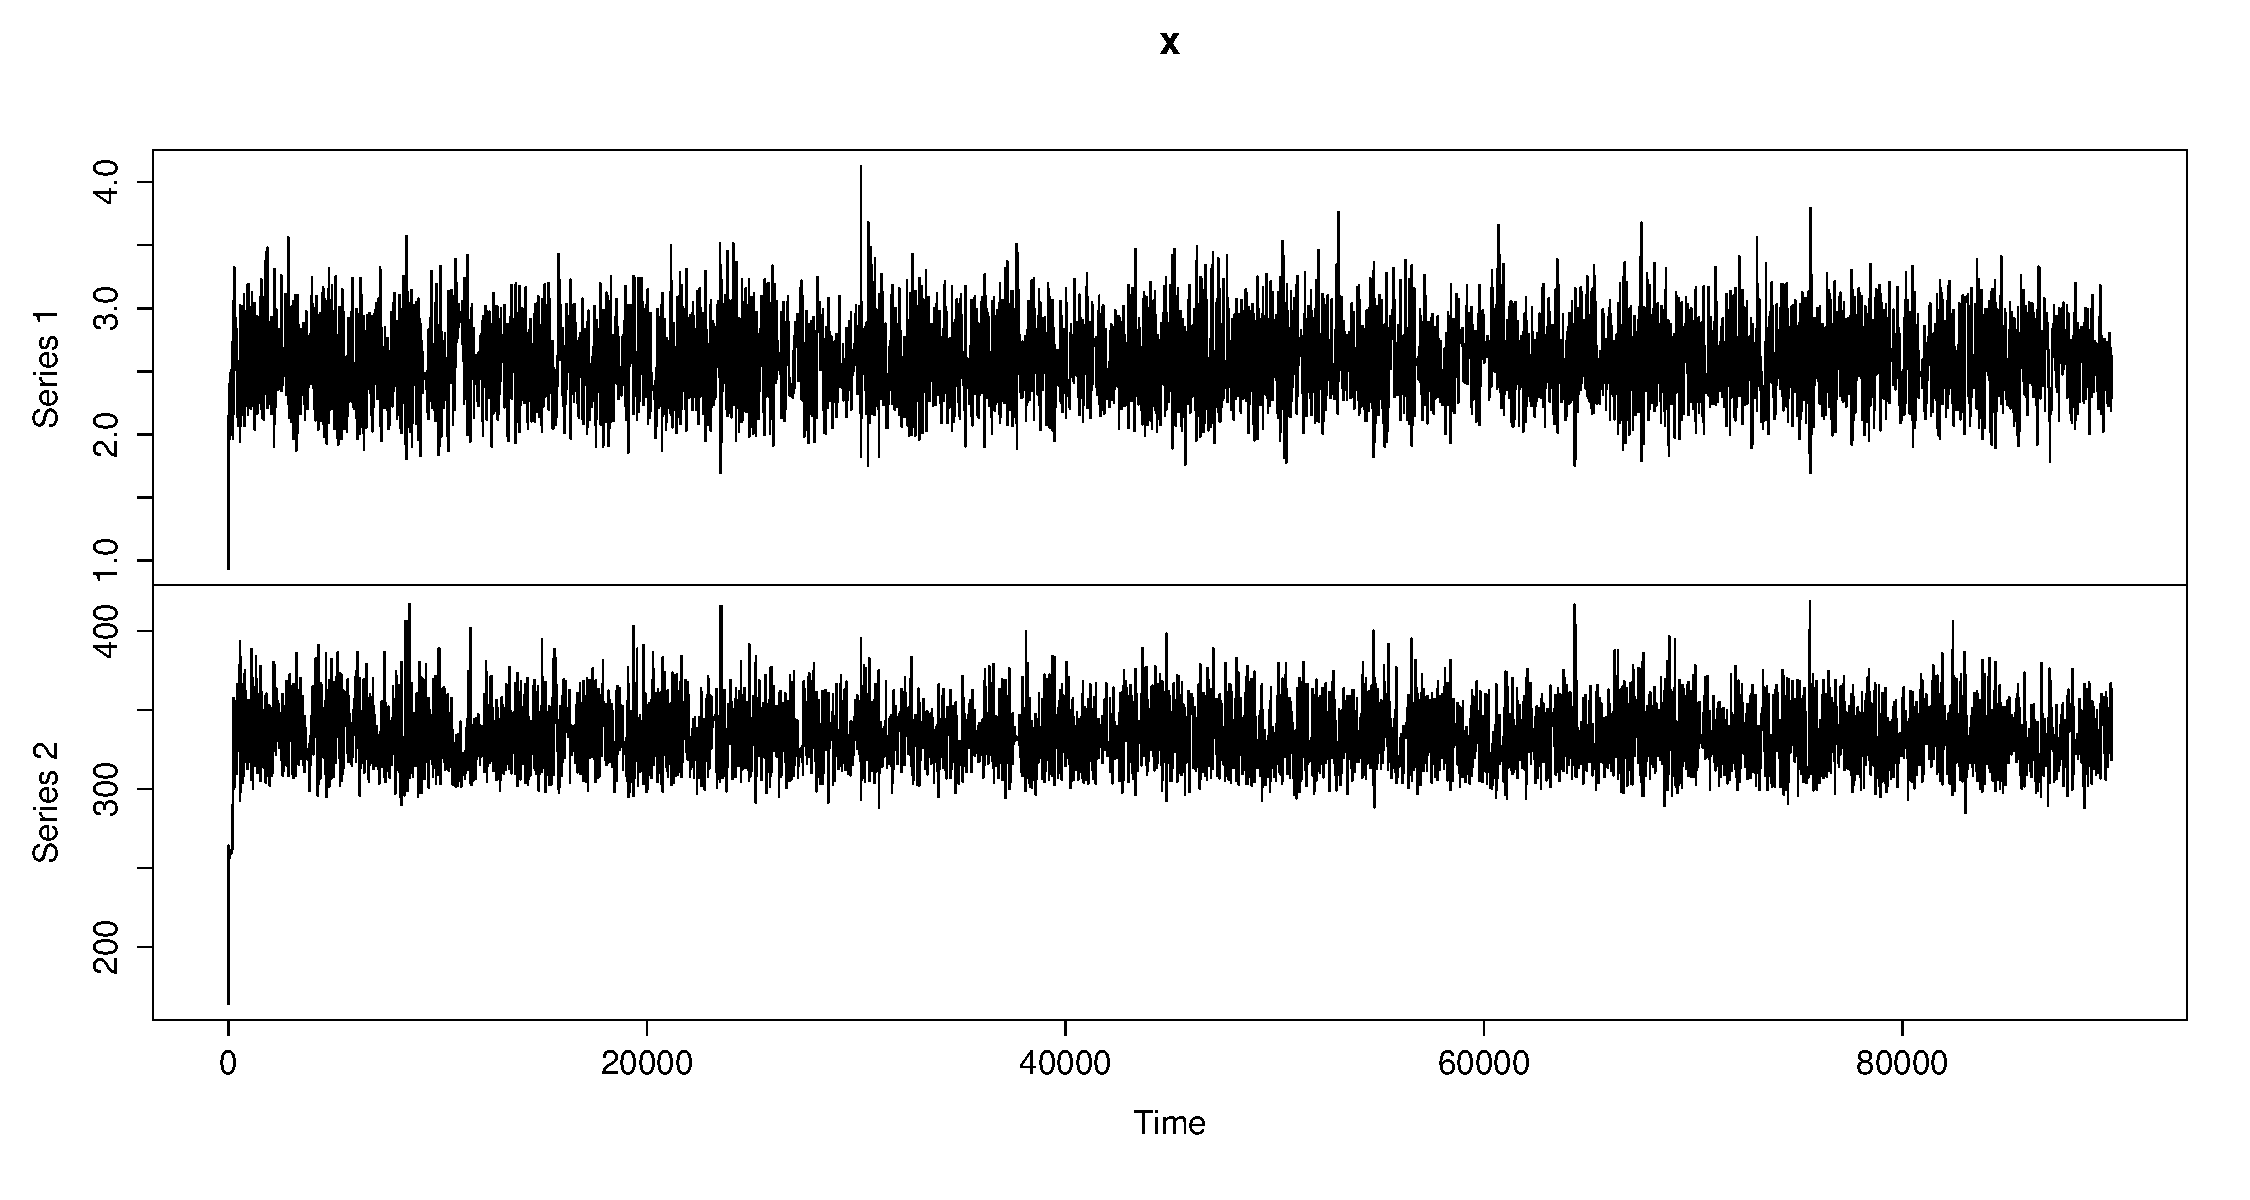
\includegraphics[scale=0.25]{serie.pdf}
\end{center}
\vspace{-1cm}\caption{{\bf Series de convergencia de los par\'ametros $\beta$ y $\eta$, proporcionados por la funci\'on t-Walk. La serie 1 corresponde a $\beta$ y la serie 2 a $\eta$.}\label{serie}}
\end{figure}

%\begin{figure}
%\begin{center}
%\includegraphics[scale=0.4]{corre1.pdf}
%\end{center}
%\vspace{-1cm}
%\caption{{\bf Muestra MCMC obtenida de la funci\'on t-Walk, graficada puntualmente con los valores de $\beta$ y $\eta$.}}
%\label{serie}
%\end{figure}

\noindent Las Figuras \ref{mlog} y \ref{serie}, muestran el an\'alisis de convergencia obtenido empleando la funci\'on t-walk. Observamos que la convergencia se da en un n\'umero de iteraciones relativamente peque\~no.\\[0.2cm]
\noindent Con la muestra, se obtiene  la densidad predictiva posterior, que describe el comportamiento de los tiempos de vida de los transformadores. La Figura \ref{apripos} muestra esta distribuci\'on, considerando la incertidumbre de los par\'ametros desconocidos $\beta$ y $\eta$.
\begin{figure}
\begin{center}
\includegraphics[scale=0.25]{DenPos.pdf}
\end{center}
\vspace{-1 cm} \caption{{\bf Densidad predictiva  posterior.}\label{apripos}}
\end{figure}


\noindent La funci\'on de confiabilidad y la funci\'on de riesgo se presentan en las Figuras \ref{CPos} y \ref{RPos} respectivamente. La confiabilidad decae lentamente. Se espera que a los 200 meses la probabilidad de que un transformador no falle es de 0.8. En la Tabla  \ref{conf} se muestran las probabilidades  de la funci\'on de confiabilidad, de los transformadores que segu\'ian operando despu\'es del 2006.

\begin{table}[h!]\small
\centering
\caption{\bf Confiabilidad de los transformadores que segu\'ian funcionando despu\'es del 2006.}\label{conf}
\vspace{.2cm}
\begin{tabular}{c|cccccc}
\toprule[0.6mm]
Meses de trabajo &8 &  20 & 32  & 56 & 80 &116  \\
\hline
Confiabilidad & 0.99 &0.99     &  0.99   &0.98 &0.97  &0.93 \\
\hline
Meses de trabajo &152 &164 &176& 188& 272& 296  \\
\hline
Confiabilidad & 0.87  &0.85   &  0.82     & 0.79 &0.55  &0.47 \\
\toprule[0.6mm]
\end{tabular}
\end{table}

\begin{figure}
\begin{center}
\includegraphics[scale=0.25]{ConPos.pdf}
\end{center}
\vspace{-0.5 cm} \caption{{\bf Confiabilidad posterior obtenida.}\label{CPos}}
\end{figure}


\noindent La probabilidad de que un transformador siga funcionando despu\'es de 8 meses es alta, de 0.99. Mientras que la probabilidad de que funcione  despu\'es de 12 a\~nos empieza a  decrecer, es de 0.87.\\
\noindent Un aspecto importante a evaluar es conocer la confiabilidad condicional, dada por: 
\vspace{-.1cm}
\begin{eqnarray*}
C(t_0|t)=P(T>t_0+t|T>t).
\end{eqnarray*}
\noindent  Esta indica la confiabilidad de un componente que ya ha vivido hasta un tiempo $t$. En la  Tabla \ref{ccc} se muestra la confiabilidad condicional de los transformadores que han vivido hasta un tiempo dado. 
\noindent Cuando el transformador ha trabajado 8 meses, la probabilidad de que siga funcionando un a\~no m\'as, es practicamente 1 y la probabilidad de que trabaje 12 a\~nos m\'as es 0.96, indicando que es un componente nuevo y su tiempo de vida es bueno, a\'un despu\'es de 12 a\~nos de operaci\'on. Por otra parte cuando un transformador ya ha vivido 308 meses (25 a\~nos), la probabilidad de que opere un a\~no m\'as es 0.4 y la probabilidad que viva 20 a\~nos m\'as es casi cero.

\begin{table}[ht]\small
\begin{center}
\caption{\bf Confiabilidad condicional de los transformadores que segu\'ian en funcionamiento despu\'es del 2006}\label{ccc}
\vspace{.3cm}
\begin{tabular}{c|c|c|c|c|c}
\toprule[0.6mm]
 Meses de trabajo ($t$) & C(1 a\~no$|t$) &C(2 a\~nos$|t$ ) &C( 7  a\~nos $|t$) & C(12 a\~nos$|t$) & C(20 a\~nos$|t$) \\ 
\toprule[0.6mm]
%\hline
  8& 1.00 & 1.00 & 0.99 & 0.98 & 0.96 \\ 
  20 & 1.00 & 1.00 & 0.98 & 0.96 & 0.91 \\ 
  32 & 0.99 & 0.99 & 0.96 & 0.93 & 0.85 \\ 
  56 & 0.98 & 0.98 & 0.92 & 0.86 & 0.73 \\ 
  80 & 0.96 & 0.95 & 0.88 & 0.78 & 0.62 \\ 
  116 & 0.92 & 0.90 & 0.79 & 0.66 & 0.47 \\ 
  152 & 0.85 & 0.83 & 0.68 & 0.54 & 0.34 \\ 
  164 & 0.82 & 0.80 & 0.65 & 0.50 & 0.30 \\ 
  176 & 0.80 & 0.77 & 0.61 & 0.46 & 0.26 \\ 
  188 & 0.76 & 0.73 & 0.57 & 0.42 & 0.23 \\ 
  272 & 0.52 & 0.48 & 0.31 & 0.19 & 0.08 \\ 
  296 & 0.44 & 0.41 & 0.25 & 0.15 & 0.06 \\ 
  308 & 0.41 & 0.37 & 0.23 & 0.13 & 0.05 \\ 
\bottomrule[0.6mm]
\end{tabular}\label{condicional}
\end{center}
\end{table}

\noindent Para obtener  los valores de la Tabla \ref{condicional}, se considera la incertidumbre de los par\'ametros desconocidos $\beta$ y $\eta$, la cu\'al se refleja por los valores obtenidos de la muestra de la distribuci\'on posterior, dada en (\ref{pos}), siendo que de (\ref{a}) y (\ref{b}), 
\begin{eqnarray*}
C(t_0|t)=\int P(T>t_0+t|T>t,\beta,\eta)f(\beta,\eta)d\beta d\eta.
\end{eqnarray*}

\noindent Dicha integral es aproximada con la muestra de la distribuci\'on generada mediante el empleo del algoritmo MCMC (t-Walk) por medio de la expresi\'on (\ref{b}). 
\noindent Para evaluar el patr\'on de desgaste de la unidades en la Figura \ref{RPos} observamos la funci\'on de riesgo de los transformadores, esta crece de manera lenta.
\begin{figure}[h!]
\begin{center}
\includegraphics[scale=.25]{Rpos.pdf}
\end{center}
\vspace{-1 cm}{\caption{\bf  Tasa de falla mensual, empleando la muestra de la funci\'on t-Walk.}\label{RPos}}
\end{figure}
\noindent Por lo tanto cabe recalcar que las gr\'aficas de las Figuras \ref{apripos}, \ref{CPos} y \ref{RPos} son aproximaciones empleando la muestra de la distribuci\'on posterior obtenida y aplicando (\ref{b}).



%\end{document}
\newpage \thispagestyle{empty} \cleardoublepage
%\input{uutilidad2.tex}

\chapter{P\'erdida Esperada}
\noindent Con frecuencia nos enfrentamos a situaciones donde debemos tomar decisiones de trascendencia, tanto de inter\'es personal como de inter\'es organizacional. La importancia  de una decisi\'on depende del riesgo asociado a ella, por lo cual es importante conocer,
tanto su probabilidad, como su costo. El proceso que conlleva una decisi\'on puede realizarse identificando adecuadamente los siguientes aspectos:

\begin{itemize}
\item Localizar el punto en donde se requiere tomar la decisi\'on.
\item Establecer una serie de hip\'otesis que pueden ser aceptadas o refutadas mediante el uso de modelos que se han dise\~nado para tal fin.
\item Conocer las consecuencias asociadas a las diferentes elecciones posibles, las cuales frecuentemente son medidas en costos monetarios.\end{itemize}


%En cualquier entorno de decisi\'on se distinguen los siguientes elementos:
%
%
%\begin{itemize}
%\item Una o mas decisiones que tienen una serie de objetivos y metas definidos.
%\item Un conjunto de acciones o alternativas disponibles para las decisiones.
%\item Un entorno de posibles resultados por la instrumentaci\'on de acciones.
%\item Una funci\'on que asocia acciones y resultados del entorno.
%\item Un proceso de decisi\'on, que selecciona una o varias acciones, dado un cierto entorno.
%\item Un criterio que marca el proceso de decisi\'on.
%
%\end{itemize}

\noindent Uno de los principales objetivos al realizar un estudio de confiabilidad, es tomar decisiones que minimicen costos. El tema de optimizaci\'on no se aborda dentro de la literatura cl\'asica de confiabilidad. Es com\'un que para pronosticar algunas cantidades de inter\'es  se consideren cuantiles adecuados, ya sean bajos o altos, seg\'un el problema que se desee resolver, omitiendo consideraciones externas como monetarias u optimizaci\'on de procesos.

\noindent Lo ideal ser\'ia decidir en forma adecuada, considerando todos los factores y prever de antemano los costos asociados a esa decisi\'on, para as\'i enfocar programas que reflejen una reducci\'on de costos.

\noindent En este trabajo se dise\~na una metodolog\'ia para la construcci\'on de un plan \'optimo de almacenamiento de transformadores. Haciendo uso de una funci\'on de p\'erdida que ser\'a definida en un contexto, que permita minimizar los costos del almac\'en.


\section{Almacenamiento de Transformadores}

\noindent Los transformadores de instrumento son herramientas costosas y dif\'iciles de transportar. La mayor\'ia de las empresas que fabrican este tipo de transformadores lo hacen bajo pedido y se tardan un tiempo considerable en cumplirlo. Su abastecimiento resulta una tarea a optimizar, debido a los costos que pueden minimizarse, como transporte y el costo del almacenamiento mismo, cuando no se usaron los aparatos. Sin embargo esta optimizaci\'on, debe ser tal que no permita que la empresa se quede sin transformadores puesto que esto implicar\'ia un costo  por no poder cobrar el servicio.

\noindent En el presente trabajo se busca desarrollar un plan de inventario para la optimizaci\'on del n\'umero de transformadores almacenados a un tiempo $t$. Para ello necesitamos tener cierta informaci\'on sobre la manera en que debe operar el almac\'en.
%, a continuaci\'on se definir\'an 

%algunas consideraciones importantes.\\[0.2cm]
\noindent Sea $n_0$ el n\'umero inicial de transformadores disponibles para reemplazar a los que fallan. Supongamos que al momento en que falla un transformador, se hace el pedido para sustituirlo y se espera un periodo de $\delta$ meses hasta que llega la orden. Mientras tanto este se reemplazar\'a por uno de los $n_0$ disponibles, si es que todav\'ia quedan en el almac\'en. Interesa determinar el valor de $n_0$, que asegure que a lo largo del periodo de tiempo analizado $(0,t)$, el almac\'en tenga los suficientes transformadores para cubrir las fallas a un costo m\'inimo.\\[0.2cm]
\noindent En el cap\'itulo anterior obtuvimos la muestra de la distribuci\'on posterior para los par\'ametros, que describen el comportamiento del tiempo de vida de los transformadores. La Figura \ref{lo} muestra un esquema representativo, de los elementos disponibles para la construcci\'on de la funci\'on de p\'erdida, que conduzca a la determinaci\'on de $n_0$.
\begin{figure}[h!]
\hspace{-2 cm}
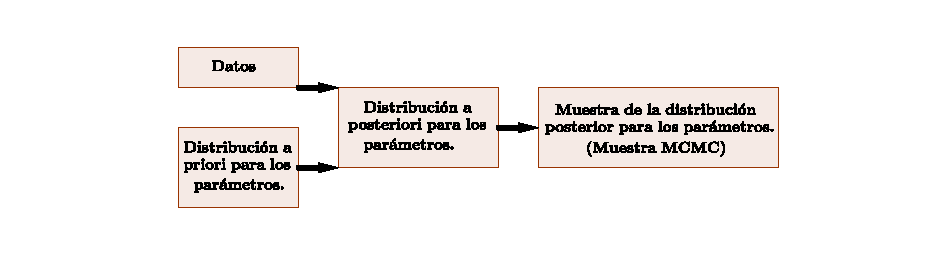
\includegraphics[scale=1.2]{esq.pdf}
\vspace{-1.5cm}\caption{\bf Etapas Realizadas en el Cap\'itulo Anterior.}\label{lo}
\end{figure}
\noindent Mientras que la Figura \ref{op} es un diagrama general de las etapas para  determinar la propuesta de inventario \'optima, empleando  la muestra de la distribuci\'on posterior y algunos costos que posteriormente estableceremos.

\begin{figure}[h!]
\hspace{-1 cm}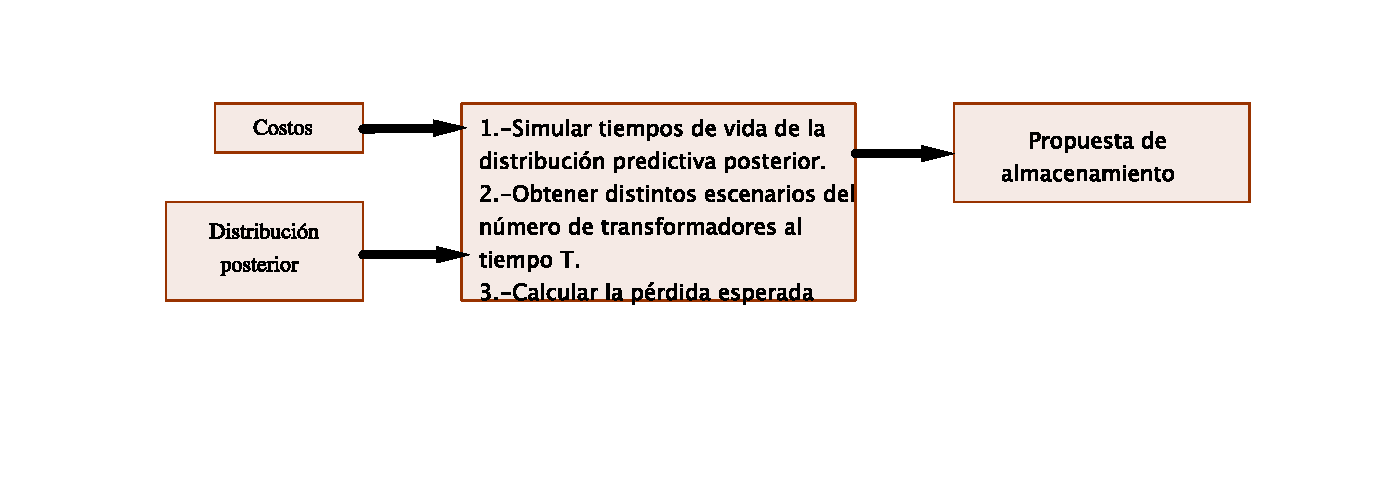
\includegraphics[scale=0.7]{final.pdf}
\vspace{-2.4 cm}\caption{\bf Contrucci\'on del Plan de Almacenamiento.}\label{op}
\end{figure}


\noindent El procedimiento  para determinar el valor \'optimo de $n_0$, se basa en el c\'alculo de la funci\'on de p\'erdida esperada. Para esto simulamos tiempos de vida $t_1,t_2,\cdots, t_n$. El tiempo $t_i$, $i=1,\cdots,n$ provendr\'a de una distribuci\'on Weibull con par\'ametros $(\beta_i,\eta_i)$ de la muestra que ya se obtuvo de la distribuci\'on posterior. Tabla \ref{ejee} contiene un conjunto de realizaciones $(\beta,\eta)$ de la distribuci\'on posterior y el $t_i$ correspondiente,

\begin{itemize}
\item $t_1=274$ es un dato que proviene de la distribuci\'on Weibull(2.228,347.37).
\item $t_2=542$ es un dato que proviene de la distribuci\'on Weibull(2.386,358.77).
\item $t_3=30.5$ es un dato que proviene de la distribuci\'on Weibull(3.534,350.55).
\item $\vdots$
\item $t_n=180$ es un dato que proviene de la distribuci\'on Weibull(2.456,340.51).
\end{itemize}
\noindent Los tiempos de vida simulados pueden ser considerados como una muestra, que resulta de una mezcla de distribuciones Weibull. Se puede demostrar que estos tiempos de vida provienen de la distribuci\'on posterior predictiva de $t$. Se calcula por medio de la siguiente integral:
\begin{eqnarray*}
f(t|\mbox{Datos})&=& \int f(t|\beta,\eta)f(\beta,\eta|\mbox{Datos})d\beta d\eta
\end{eqnarray*}

y se aproxima por medio de (\ref{c}).



\begin{table}
\begin{center}

\vspace{-.3 cm}\caption{\bf Muestra MCMC.}\label{ejee}
\vspace{0.3cm}\begin{tabular}{cccc}
\toprule[0.6mm]
$i$&$\beta$ &$\eta$& $t_i$\\\toprule[0.6mm]
1&2.228 & 347.37 & 274
\\ 2&2.386 & 358.77 & 542
\\3&3.534 & 350.55 &305\\
 $\vdots$&$\vdots$ & $\vdots$ &$\vdots$
\\$n$& 2.456 & 340.51 & 180\\
\toprule[0.6mm]
\end{tabular}
\end{center}

\end{table}
\newpage

%\item {\bf Obtenci\'on de distintos escenarios del n\'umero de transformadores en el almac\'en}

\noindent Una vez establecidos los tiempos de falla de los transformadores. El n\'umero de transformadores en el almac\'en hasta el  tiempo $t$, depender\'a del n\'umero de fallas que ocurran durante el periodo de observaci\'on $(0,t)$, de $\delta$ y del n\'umero de transformadores que fijemos como iniciales $n_0$, es decir, es una funci\'on: $$n(t,n_0,\delta).$$
\noindent Para observar el comportamiento de $n(t,n_0,\delta)$ por simulaci\'on, se consideran tiempos de falla similares a los de la  Tabla \ref{ejee}. Se asume que al momento en que falla un transformador se solicita y llega $\delta$ meses despu\'es. Como solo se pide un transformador cuando alguno ha fallado, siempre tendremos en el almac\'en a lo m\'as $n_0$ transformadores.
\noindent De manera m\'as clara la forma de operar de $n(t,n_0,\delta)$, el n\'umero de transformadores disponibles en el almac\'en en el intervalo de tiempo de  $(0,t)$ es la siguiente: Al inicio del periodo $n(0,n_0,\delta)=n_0$, una vez que se llega a un tiempo de falla $t_1$ el valor de $n(t_1,n_0,\delta)$ ser\'a $n_0-1$ disminuye en uno y este se recuper\'a $\delta$ meses despu\'es. Si se llega a otro tiempo de falla antes de que llegue la orden entonces $n(\cdot)$ disminuir\'a en uno nuevamente, si ocurre lo contrario se recuperar\'a al menos en una unidad.\\[0.1cm]

\noindent Las gr\'aficas de algunas trayectorias simuladas de la funci\'on $n(t,n_0,\delta)$ para valores de $\delta=6,8$ y 12 meses  se muestran en las Figuras \ref{d6} \ref{d8} y \ref{d12}.

 \noindent Se decidi\'o analizar estos valores de $\delta$ , debido a que si los transformadores llegan en periodos menores de 6 meses, los valores de $n(t,n_0,\delta)$ no var\'ian de manera significativa. Por otro lado considerar periodos de espera m\'as largos que un a\~no parece ser un periodo grande de espera. 
\noindent Necesitamos establecer una funci\'on de p\'erdida, a partir de los escenarios simulados,  que permita saber la cantidad inicial adecuada de transformadores que deben tenerse en el almac\'en. La siguiente secci\'on describir\'a la manera de establecer esta funci\'on.


%\end{itemize}
%Rplot06
\begin{figure}
\begin{center}
\includegraphics[scale=.3]{Rplot06.pdf}
\end{center}
\vspace{-1 cm} \caption{\bf Dos trayectorias obtenidas mediante simulaci\'on del n\'umero de transformadores en el almac\'en hasta el tiempo $t=200$ meses,  con $n_0=5$ transformadores al inicio del periodo de observaci\'on y $\delta=6$ meses de espera de llegada de los transformadores que se han pedido.}\label{d6}
\end{figure}
\vspace{-1.5cm}
\begin{figure}
\begin{center}
\includegraphics[scale=.3]{Rplot08.pdf}
\end{center}
\vspace{-1 cm}\caption{\bf Dos trayectorias obtenidas mediantes simulaci\'on del n\'umero de transformadores en el almac\'en hasta el tiempo $t=200$, con $n_0=7$ y $\delta=8$}\label{d8}
\end{figure}

\begin{figure}
\begin{center}
\includegraphics[scale=0.3]{Rplot10.pdf}
\end{center}
\vspace{-1 cm}\caption{\bf Trayectorias simuladas del n\'umero de transformadores en inventario o almacenados con $n_0=10$, $t=200$ y $\delta=12.$}\label{d12}
\end{figure}


\section{Funciones de P\'erdida}

\noindent Al hablar de funci\'on de p\'erdida nos referimos a una funci\'on que expresa los costos de p\'erdidas o ganancias  al tomar diferentes acciones. A continuaci\'on se proponen tres posibles pol\'iticas de inventario y posteriormente se describen sus funciones de p\'erdida. Se considera una pol\'itica de inventario, al planteamiento de una funci\'on de p\'erdida que refleje los costos de mayor inter\'es para la empresa.



\begin{description}
\item [Pol\'itica A] \hfill \\ 
La primera pol\'itica reflejar\'a el costo de quedarnos sin transformadores disponibles en el almac\'en. Estar\'a  enfocada a determinar el $n_0$ adecuado, tal que no permita que dentro del periodo de observaci\'on, el almac\'en se quede sin transformadores para cubrir todas sus demandas.
\item [Pol\'itica B] \hfill \\
La segunda pol\'itica adem\'as de considerar el costo de la pol\'itica A, adiciona el costo del lote inicial de transformadores en el almac\'en. 
\item [Pol\'itica C] \hfill \\
Esta \'ultima pol\'itica se centra en evaluar dos tipos de costos.
\begin{itemize}
\item[1.-] Costo de falta de transformadores por unidad de tiempo. Este costo tambi\'en considerado en las pol\'iticas anteriores.
\item[2.-] Costo de almacenamiento por cada unidad de tiempo.
\end{itemize}
\end{description}

\subsection{Pol\'itica A}

\noindent Usando las Figuras \ref{d6} \ref{d8} y \ref{d12}, es posible obtener la permanencia por debajo de cero de las trayectorias para distintos valores iniciales de $n_0$, lo cual se interpretar\'ia como el n\'umero de veces que la empresa se quedo sin transformadores para reemplazar. Es natural que entre m\'as peque\~no sea $n_0$, se permanece m\'as tiempo por debajo de cero y entre m\'as grande, la empresa se quedar\'a sin reservas por menos tiempo.\\[0.1cm]
\noindent Supongamos que se tiene una trayectoria como la de la Figura \ref{tr}, hasta un tiempo de $10$ meses y con $1$ transformador inicial de reserva. Supongamos adem\'as que al tiempo 3 falla un transformador, luego  $n(3)=0$. Despu\'es de un tiempo falla otro y no tenemos repuesto, entonces el n\'umero de transformadores en reserva es negativo ($n(4)=-1$). La p\'erdida asociada a partir de este tiempo, es el n\'umero de meses que permanece en esta situaci\'on (1 mes), multiplicada por un valor de $c$ unidades monetarias, que representa el costo de no poder cobrar la electricidad, por cada mes que no se tuvo un transformador de instrumento. Si se observa hasta $t=10$ entonces habr\'ia que sumar las p\'erdidas que representan el segundo bloque, que empieza en el tiempo $t=6$. Del bloque de $t=6$ a $t=7$ la p\'erdida involucra solamente a un transformador. Sin embargo en el intervalo de tiempo de $[7,9]$ meses la p\'erdida es m\'as grande, puesto que faltan dos transformadores para sustituir. La p\'erdida  ser\'a  los dos transformadores faltantes multiplicada por la longitud de tiempo que dure este hecho, (2 meses) por el valor de $c$. Por lo tanto la p\'erdida  total es:
\begin{eqnarray*}
c[1\cdot1 + 1\cdot1+2\cdot2+1\cdot1]
\end{eqnarray*} 
Lo que significa que la p\'erdida es la suma de las \'areas delimitadas por debajo de cero, multiplicada por $c$, donde $c$ se tiene que establecer con informaci\'on adicional. Sin perder generalidad se puede suponer $c=1$.\\[0.2cm]

\begin{figure}[h!]
\begin{center}
%\includegraphics[width=10cm,height=5cm]{Rplot01.png}
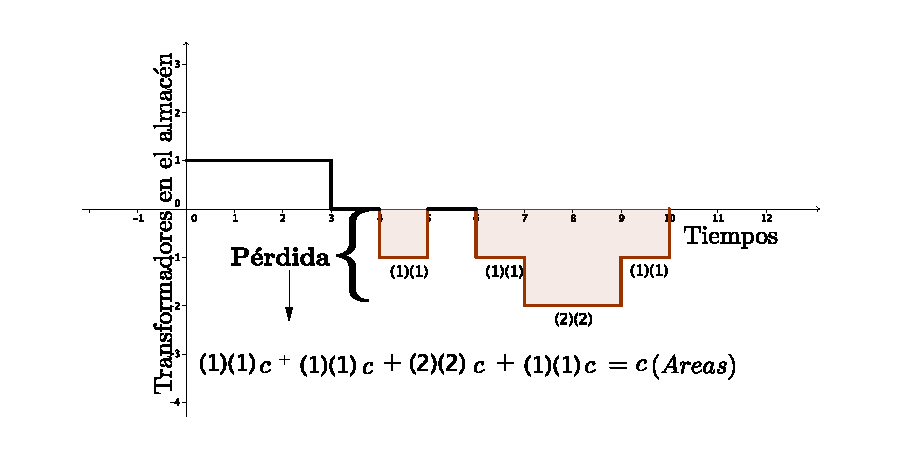
\includegraphics[scale=1]{tr1.pdf}
\end{center}
\vspace{-1.5 cm} \caption{\bf Almacenamiento de transformadores, hasta $10$ unidades de tiempo, mostrando la p\'erdida sobre ese per\'iodo.}\label{tr}
\end{figure}



\noindent De manera  general, podemos construir la funci\'on de p\'erdida asociada a la pol\'itica A, como se describe a continuaci\'on.\\[0.2cm]
\noindent Sean $\underline{T}=\{t_1,t_2,\cdots,t_n\}$ los tiempos de falla de los transformadores y 
$\underline{\ell}=\{\ell_1=t_1+\delta, \ell_2=t_2+\delta, \cdots, \ell_n=t_n+\delta\},$ los tiempos de llegada de los transformadores pedidos. 

\noindent  Definamos  $X(t;\underline{T})$ como el  n\'umero de transformadores en el almac\'en que se usaron para cubrir los tiempos de fallas hasta el tiempo $t$ y  $Y(t;\underline{T})$ el n\'umero de transformadores que se pidieron y llegaron antes del tiempo $t$. Luego $X(0)=n_0$ y $Y(0)=0$.\\[0.1cm]
\noindent Sea $Z(t,\underline{T})=X(t;\underline{T})+Y(t;\underline{T})$, indica el comportamiento de la funci\'on $n(t,n_0,\delta)$. Interesa conocer las veces en la cual esta permanece por debajo de cero.\\[0.1cm] 
\noindent La siguiente funci\'on restringue solo al \'area de inter\'es 
\[
W(t;\underline{T})=\left\{
\begin{array}{cl}
\displaystyle 0 & \mbox{ si } Z(t;\underline{T})\geq 0,\\                                                               Z(t)      &     \mbox{ si } Z(t;\underline{T})< 0  \\
\end{array}
\right.
\]

\noindent Una vez establecidas las funciones anteriores la funci\'on de p\'erdida esta dada por 

\begin{eqnarray}\label{LL}
L(t,\underline{T};\delta, n_0)=\int_{0}^{t} W(s;\underline{T}) ds,
\end{eqnarray}

\noindent dicho en palabras la p\'erdida esta representada por la integral sobre el periodo de observaci\'on, de las veces en las cuales el almac\'en se quedo sin transformadores disponibles para su uso.\\[0.1cm]
Para tener una idea clara de la forma de calcular (\ref{LL}), veamos el siguiente que ejemplo.\\[0.1cm]
 %Para $\underline{T}$, $Z(t)$ \\[0.2cm]


{\bf \noindent  Ejemplo:} 
\\[0.1cm]
Supongamos que en el intervalo $(0,7)$ de tiempo, ocurrieron solo 6 fallas, en los tiempos dados en la Tabla \ref{4500}. Es de inter\'es  conocer el n\'umero de transformadores al tiempo 7 con $n_0=3$ y $\delta=3$.
\begin{table}[h!]\small
\caption{\bf Valores de \underline{T}.\label{4500}}
\centering
\vspace{0.3cm }\begin{tabular}{cccccc}
\toprule[0.6mm]
0.730 & 0.812 & 0.868 &  2.786 &  3.064 &  3.401  \\
\toprule[0.6mm]
\end{tabular}
\end{table}


\noindent La Figura \ref{ejeu1} muestra dos gr\'aficas, la primera de lado izquierdo, ilustra a trav\'es del tiempo la forma de comportarse del n\'umero de  transformadores que se usaron para cubrir los tiempos de falla. Por cada tiempo de falla, el n\'umero de transformadores en el almac\'en disminuye en 1. Dado que iniciamos con 3 transformadores $X(0)=3$, al final de la sexta  falla $X(3.401)=-3$. 




\begin{figure}[h!]
\begin{center}
\includegraphics[scale=.35]{ejeu1.pdf}
\end{center}
\vspace{-1 cm} \caption {\bf Izquierda: Funci\'on $X(t)$ el n\'umero de transformadores en el almac\'en que se usaron para cubrir las fallas durante el periodo de observaci\'on. Derecha: Funci\'on $Y(t)$, describe los tiempos en que llegaron los transformadores que fueron solicitados.}\label{ejeu1}
\end{figure}

\noindent Mientras que del lado derecho vemos el comportamiento de $Y(t)$. Al tiempo cero, $Y(0)=0,$ ya que  no se ha pedido ning\'un transformador. La primera llegada ocurrir\'a al tiempo $t_1+\delta=0.730+3=3.730$, de ah\'i subir\'a cada $t_i+\delta$, donde los $t_i$'s son tomados de la Tabla \ref{4500}.  La  Tabla  \ref{23} muestra los tiempos en los cuales llegaron los transformadores pedidos.
\begin{table}[h!]\small
\centering
\caption{\bf Valores de $\underline{\ell.}$}\label{23}
\vspace{0.3cm }\begin{tabular}{cccccc}
\toprule[0.6mm]
3.730 & 3.812 & 3.868 &  5.786 &  6.064 &  6.401  \\
\toprule[0.6mm]
\end{tabular}

\end{table}



 \noindent Una vez teniendo estas gr\'aficas podemos obtener $Z(t)$ como la suma de ellas, mostrada en la Figura \ref{ejeu2}, esta gr\'afica representa los tiempos a los cuales fallaron los transformadores y llegaron los repuestos, de acuerdo a las Tablas \ref{4500} y \ref{23}. 

\begin{figure}[h!]
\begin{center}
\includegraphics[scale=.3]{ejeu2.pdf}
\end{center}
\vspace{-1 cm} \caption{\bf Funci\'on $Z(t)$ es el n\'umero de transformadores el almac\'en hasta $t=7.$}\label{ejeu2}
\end{figure}

\noindent El tiempo de permanencia sin transformadores y durante que periodos se observa en la Figura \ref{ejeu3},  representada por la funci\'on $W(t)$. Esta funci\'on es escalonada baja y sube seg\'un fue un tiempo de falla o un tiempo de llegada de un transformador pedido. Los valores expl\'icitos de $W(t)$, est\'an en la Tabla \ref{dosa}.

 
 
 \begin{figure}[h!]
\begin{center}
\includegraphics[scale=.3]{ejeu3.pdf}
\end{center}
\vspace{-1 cm}\caption{\bf Funci\'on $W(t)$ que representa la trayectoria negativa de los transformadores en el almac\'en.}\label{ejeu3}
\end{figure}


 
\begin{table}[h!]\small
\centering
\caption{\bf Valores de la funci\'on $W(t)$.}\label{dosa}
\begin{tabular}{ccccccc}
\toprule[0.6mm]
Tiempos&0.730& 0.812 & 0.868 &  2.786 &  3.064&  3.401  \\\hline
$W$(Tiempos) & 0  &0      &  0     & -1 &-2  &-3 \\
\hline
Tiempos&3.730 & 3.812 & 3.868 &  5.786 &  6.064&  6.401  \\\hline
$W$(Tiempos) & -2  &-1    &  0     & 0 &0  &0 \\
\toprule[0.6mm]
\end{tabular}

\end{table}

\newpage
 
\noindent  La funci\'on de p\'erdida dada en la Ecuaci\'on (\ref{LL}), se obtiene como el \'area de la funci\'on $W(t)$.

\begin{eqnarray*} 
L(\underline{T},3,3)&=&\int W(s) ds\\
&=& 1( 3.064-2.786)+ 2(3.401-3.064)+3(3.730- 3.401)\\
&+&2( 3.812- 3.730)+ 1(3.868-3.812)\\
&=&8.159
\end{eqnarray*}

\noindent Por lo tanto el valor de la funci\'on de p\'erdida es $8.159$.

\subsubsection{P\'erdida Esperada}

\noindent La funci\'on de p\'erdida dada por la Ecuaci\'on (\ref{LL}), depende de $n_0$, $\delta$ que son valores constantes y de \underline{T} que es una variable aleatoria, por lo tanto la funci\'on de p\'erdida es una funci\'on estoc\'astica, en el sentido de que depende de una variable aleatoria. Entonces la p\'erdida esperada tambi\'en es una funci\'on estoc\'astica, y esta dada por:
\begin{eqnarray}\label{ut}
U(t,n_0,\delta)=E(L(t,\underline{T},n_0, \delta)).
\end{eqnarray}

\noindent Por la ley de los grandes n\'umeros, la manera de estimar la Ecuaci\'on (\ref{ut}), es mediante la  expresi\'on:

\begin{eqnarray}\label{utqq}
\hat{U}(t,n_0,\delta)=\frac{1}{M} \sum_{s=1}^{M}\int_{0}^{t} W(y,\underline{T}_s) dy,
\end{eqnarray}
 donde $M$ es el n\'umero de $\underline{T}_s$ simulados.
\noindent Para calcular la expresi\'on (\ref{utqq}) por simulaci\'on se hace de la siguiente manera:

\begin{enumerate}
\item Se simulan $M$ trayectorias de tiempos de vida, dicho en otras palabras $M$ vectores del tipo $\underline{T}$.
\item Para cada trayectoria se calcula la Ecuaci\'on (\ref{LL}).
%que indica la p\'erdida en toda la trayectoria de tiempos simulada.
\item De los $M$ valores obtenidos,  se obtiene el promedio de ellos, que ser\'a la p\'erdida esperada.
%\item Una vez que se tienen las $M$, trayectorias y sus sumas asociadas, se calcula el promedio de las sumas, los cuales representan la p\'erdida esperada (Ecuaci\'on \ref{utqq}).\\[0.2cm]
\end{enumerate}

\noindent De acuerdo a los pasos anteriores, se realizaron 1000 simulaciones para cada pareja $$(\delta_i,n_{0_j})$$ donde $\delta_i=6, 8$ y 12 meses, $n_{0_j}=1,2,\cdots, 24$ que representa el n\'umero de transformadores al inicio del periodo. Luego se obtuvo el promedio de las funciones de p\'erdida, calculadas en cada una de las 1000 simulaciones para cada pareja, se consider\'o un tiempo de observaci\'on de 40 a\~nos (480 meses).\\[0.1cm]

\noindent La Figura \ref{d6s} muestra la gr\'afica de las p\'erdidas esperadas para $\delta=6,8,12$ meses.  Observamos que para valores de $n_0$ peque\~nos, 
las perdidas esperadas son grandes. A medida que $n_0$ crece, los promedios disminuyen. Al considerarse tiempos de espera m\'as largos, los costos tambi\'en se incrementan, las mayores p\'erdidas se tienen cuando $\delta=12$, para este periodo de espera se necesitan al menos 24 transformadores al inicio del periodo de observaci\'on (Tabla \ref{c777}). Para $\delta=8$ se requieren 15 transformadores (Tabla  \ref{c33333} )y para $\delta=6$ se necesitan 15 transformadores en el almac\'en (Tabla \ref{c1}).



\begin{figure}[h!]
\begin{center}
\includegraphics[scale=0.35]{poA.pdf}
\end{center}
\vspace{-1 cm} \caption{\bf P\'erdidas Esperadas con la Pol\'itica A, usando $t=480$, $\delta=6,8,12$ y Differentes Valores de $n_0$.}\label{d6s}
\end{figure}


%\begin{figure}[h!]
%\begin{center}
%\includegraphics[scale=0.25]{u6.pdf}
%\end{center}
%\vspace{-1 cm} \caption{\bf  p\'erdidaes esperadas con la pol\'itica A usando $t=480$ y $\delta=6$}\label{d6s}
%\end{figure}

\begin{table}[h!]\small
\centering
\caption{\bf Pol\'itica A: Valores de las P\'erdidas Esperadas con $\delta=6$.}\label{c1}
\vspace{0.3 cm}\begin{tabular}{ccccccccc}
\toprule[0.6mm]

$\bf{n_0}$&\bf{1} &                   \bf{2} &                   \bf{3} &                   \bf{ 4 }&                    \bf{ 5}&              \bf{ 6} &               \bf{ 7} & \bf{8} \\
\hline
$\mbox{\bf Promedio}$&1029.433  &697.822&  437.725&  251.263 & 131.085 &  62.514 &  27.148 &  11.136 \\	
\hline
$\bf{n_0}$&\bf{9} &                \bf{ 10}&              \bf{      11} &                   \bf{ 12} &               \bf{      13}&              \bf{14} &  \bf{ 15} & \bf{16 }   \\
\hline
$\mbox{\bf Promedio}$&	 4.003  &  1.343 &   0.446 &   0.167&    0.028 &   0.040 &   0.000&    0.000\\ 
	 \hline
	
$\bf{n_0}$&\bf{17} &     \bf{ 18}&   \bf{19}&   \bf{ 20} &           \bf{   21}&                \bf{  22}  & \bf{23} & \bf{24}  \\
\hline
$\mbox{\bf Promedio}$&  0.000 &   0.000&    0.000 &   0.000   & 0.000  &  0.000 &   0.000 & 0.000\\
\toprule[0.6mm]
\end{tabular}

\end{table}
%------------------------------------------------------------------------------------------------------------------------------------------------------------
%delta=7

%\begin{figure}
%\begin{center}
%\includegraphics[width=9cm,height=5cm]{delta7t480sumas.pdf}
%\end{center}
%\vspace{0.01 cm} \textsl{\caption{$n_0$ toma valores de 1 hasta 23, $t=480$ y $\delta=7$}\label{d7s}}
%\end{figure}
%
%
%\begin{table}[h!]
%\centering
%\begin{tabular}{|c|c|c|c|c|c|c|c|c|}
%\hline
%$\bf{n_0}$&\bf{1} &                   \bf{2} &                   \bf{3} &                   \bf{ 4 }&                    \bf{ 5}&              \bf{ 6} &               \bf{ 7} & \bf{8} \\
%\hline
%$Promedio$&1253.239 & 899.652 & 609.664 & 385.596&  223.191&  118.834 &  59.093  & 26.753\\ 
%\hline
%$\bf{n_0}$&\bf{9} &                \bf{ 10}&              \bf{      11} &                   \bf{ 12} &               \bf{      13}&              \bf{14} &  \bf{ 15} & \bf{16 }   \\
%\hline
%$Promedio$&	  10.901  &  4.472&    1.427 &   0.603  &  0.151 &   0.069&    0.012 &   0.000 \\
%	 \hline
%	
%$\bf{n_0}$&\bf{17} &     \bf{ 18}&   \bf{19}&   \bf{ 20} &           \bf{   21}&                \bf{  22}  & \bf{23} &  \\
%\hline
%$Promedio$&   0.000 &   0.000&    0.000 &   0.000   & 0.000  &  0.000 &   0.000 & \\
%   \hline
%\end{tabular}
%\caption{Valores obtenidos con $\delta=7$.}\label{c2}
%\end{table}
%
%
%
%-------------------------------------------------------------------------------------------------------------------------------------------------------------
%Delta=8

%\begin{figure}[h!]
%\begin{center}
%\includegraphics[scale=0.25]{u8.pdf}
%\end{center}
%\vspace{-1 cm} \caption{\bf p\'erdidaes esperadas con la pol\'itica A, usando $t=480$ y $\delta=8$}\label{d8ssss}
%\end{figure}


\begin{table}[h!]\small
\centering
\caption{\bf Pol\'itica A: Valores de las P\'erdidas Esperadas con $\delta=8$.}\label{c33333}
\vspace{0.3 cm}\begin{tabular}{ccccccccc}
\toprule[0.6mm]
$\bf{n_0}$&\bf{1} &                   \bf{2} &                   \bf{3} &                   \bf{ 4 }&                    \bf{ 5}&              \bf{ 6} &               \bf{ 7} & \bf{8} \\
\hline
$\mbox{\bf Promedio}$&1483.721 &1118.711  &799.610  &539.082 & 338.785  &200.591  &109.192  & 55.774 \\
\hline
$\bf{n_0}$&\bf{9} &                \bf{ 10}&              \bf{      11} &                   \bf{ 12} &               \bf{      13}&              \bf{14} &  \bf{ 15} & \bf{16 }   \\
\hline
$\mbox{\bf Promedio}$&	   25.935  & 11.184  &  4.376  &  1.637   & 0.733   & 0.219   & 0.081  &  0.032  \\
	 \hline
	
$\bf{n_0}$&\bf{17} &     \bf{ 18}&   \bf{19}&   \bf{ 20} &           \bf{   21}&                \bf{  22}  & \bf{23} & \bf{24}  \\
\hline
$\mbox{\bf Promedio}$&   0.004 &   0.003&    0.000 &   0.000   & 0.000  &  0.000 &   0.000 & 0.00\\
\toprule[0.6mm]
\end{tabular}

\end{table}
%----------------------------------------------------------------------------------------------------------------------------------------------------------


%Delta=9
%
%\begin{figure}
%\begin{center}
%\includegraphics[width=9cm,height=5cm]{delta9sumas.pdf}
%\end{center}
%\vspace{0.01 cm} \textsl{\caption{$n_0$ toma valores de 1 hasta 23, $t=480$ y $\delta=9$}\label{d9s}}
%
%\end{figure}
%
%\newpage
%
%
%\begin{table}[h!]
%\centering
%\begin{tabular}{|c|c|c|c|c|c|c|c|c|}
%\hline
%$\bf{n_0}$&\bf{1} &                   \bf{2} &                   \bf{3} &                   \bf{ 4 }&                    \bf{ 5}&              \bf{ 6} &               \bf{ 7} & \bf{8} \\
%\hline
%$Promedio$&1712.065 &1336.411 &1002.302  &713.153 & 478.761  &305.225 & 182.174 & 102.668  \\
%\hline
%$\bf{n_0}$&\bf{9} &                \bf{ 10}&              \bf{      11} &                   \bf{ 12} &               \bf{      13}&              \bf{14} &  \bf{ 15} & \bf{16 }   \\
%\hline
%$Promedio$&	   51.848 &  24.706  & 10.936 &   4.594 &   1.861 &   0.721   & 0.218   & 0.072   \\
%	 \hline
%	
%$\bf{n_0}$&\bf{17} &     \bf{ 18}&   \bf{19}&   \bf{ 20} &           \bf{   21}&                \bf{  22}  & \bf{23} &  \\
%\hline
%  $Promedio$& 0.039 &   0.010&    0.002 &   0.000   & 0.000  &  0.000 &   0.000 & \\
%   \hline
%\end{tabular}
%\caption{Valores obtenidos con $\delta=9$.}\label{c4}
%\end{table}
%
%%----------------------------------------------------------------------------------------------------------------------------------------------------------
%%Delta=10
%
%\begin{figure}
%\begin{center}
%\includegraphics[width=9cm,height=5cm]{delta10sumas.pdf}
%\end{center}
%\vspace{0.01 cm} \textsl{\caption{$n_0$ toma valores de 1 hasta 23, $t=480$ y $\delta=10$}\label{d10s}}
%
%\end{figure}
%\newpage
%
%\begin{table}[h!]
%\centering
%\begin{tabular}{|c|c|c|c|c|c|c|c|c|}
%\hline
%$\bf{n_0}$&\bf{1} &                   \bf{2} &                   \bf{3} &                   \bf{ 4 }&                    \bf{ 5}&              \bf{ 6} &               \bf{ 7} & \bf{8} \\
%\hline
%$Promedio$&1944.634 & 1560.876 &1210.653 &  905.893  & 642.491 &  436.292 &  273.966  &  167.279  \\
%\hline
%$\bf{n_0}$&\bf{9} &                \bf{ 10}&              \bf{      11} &                   \bf{ 12} &               \bf{      13}&              \bf{14} &  \bf{ 15} & \bf{16 }   \\
%\hline
%$Promedio$&	   91.176  &  48.178 &  23.693 &  11.076  &  4.752 &   2.030 &   0.759 &   0.400   \\
%	 \hline
%	
%$\bf{n_0}$&\bf{17} &     \bf{ 18}&   \bf{19}&   \bf{ 20} &           \bf{   21}&                \bf{  22}  & \bf{23} &  \\
%\hline
% $Promedio$&  0.069 &   0.026&    0.006 &   0.000   & 0.000  &  0.001 &   0.000 & \\
%   \hline
%\end{tabular}
%\caption{Valores obtenidos con $\delta=10$.}\label{c5}
%\end{table}
%%-----------------------------------------------------------------------------------------------------------------------------------------------------------
%%Delta=11
%
%\begin{figure}
%\begin{center}
%\includegraphics[width=9cm,height=5cm]{delta11sumas.pdf}
%\end{center}
%\vspace{0.01 cm} \textsl{\caption{$n_0$ toma valores de 1 hasta 23, $t=480$ y $\delta=11$}\label{d11s}}
%\end{figure}
%\newpage
%\begin{table}[h!]
%\centering
%\begin{tabular}{|c|c|c|c|c|c|c|c|c|}
%\hline
%$\bf{n_0}$&\bf{1} &                   \bf{2} &                   \bf{3} &                   \bf{ 4 }&                    \bf{ 5}&              \bf{ 6} &               \bf{ 7} & \bf{8} \\
%\hline
%$Promedio$&2173.671 &1781.718& 1427.693 &1098.406  &  819.975  & 583.561  &391.518 & 248.187   \\
%\hline
%$\bf{n_0}$&\bf{9} &                \bf{ 10}&              \bf{      11} &                   \bf{ 12} &               \bf{      13}&              \bf{14} &  \bf{ 15} & \bf{16 }   \\
%\hline
%$Promedio$&	151.415 &  84.731 &  46.088 &  23.408 &  10.532 &   5.272 &   2.169 &   0.823    \\
%	 \hline
%	
%$\bf{n_0}$&\bf{17} &     \bf{ 18}&   \bf{19}&   \bf{ 20} &           \bf{   21}&                \bf{  22}  & \bf{23} &  \\
%\hline
%$Promedio$&    0.325 &   0.093  &  0.055 &   0.011  & 0.000  &  0.001 &   0.000 & \\
%   \hline
%\end{tabular}
%\caption{Valores obtenidos con $\delta=11$.}\label{c6}
%\end{table}
%
%
%%-----------------------------------------------------------------------------------------------------------------------------------------------------------
%Delta=12
%\begin{figure}[h!]\small
%\begin{center}
%\includegraphics[scale=0.25]{u12.pdf}
%\end{center}
%\vspace{-1 cm}\caption{\bf p\'erdidaes esperadas con la pol\'itica A usando $t=480$ y $\delta=12$}\label{d12s}

%\end{figure}

\begin{table}[h!]\small
\centering
\caption{\bf Pol\'itica A: Valores de las P\'erdidas Esperadas con $\delta=12$.}\label{c777}
\vspace{.3cm}\begin{tabular}{ccccccccc}
\toprule[0.6mm]
$\bf{n_0}$ &\bf{1} &                   \bf{2} &                   \bf{3} &                   \bf{ 4 }&                    \bf{ 5}&              \bf{ 6} &               \bf{ 7} & \bf{8} \\
\hline
{\bf Promedio} & 2411.0  & 2008.7 &1640.9 &1305.0&1002.0 & 740.5 & 526.5 & 357.3    \\
\hline
$\bf{n_0}$&\bf{9} &                \bf{ 10}&              \bf{      11} &                   \bf{ 12} &               \bf{      13}&              \bf{14} &  \bf{ 15} & \bf{16 }   \\
\hline
{\bf Promedio}&	 222.7 & 137.1 &  78.0 &   41.8 &  21.1  &   9.8  &    4.8  &  2.3    \\
	 \hline
	
$\bf{n_0}$&\bf{17} &     \bf{ 18}&   \bf{19}&   \bf{ 20} &           \bf{   21}&                \bf{  22}  & \bf{23} &\bf {24}  \\
\hline
   {\bf Promedio} &  0.9    &  0.34 &   0.09 &   0.03 &   0.01 &   0.02 &   0.003  & 0.00\\
\toprule[0.6mm]
\end{tabular}

\end{table}
%------------------------------------------------------------------------------------------------------------------------------------------------------------
\newpage
\noindent Cabe destacar que los valores considerandos de $\delta$'s y $t=480$ meses, se utilizaron para  ilustrar la metodolog\'ia sugerida, puesto que no se tiene acceso a los valores reales. Sin embargo con la metodolog\'ia propuesta, cualesquiera que fueran los valores reales, los c\'alculos anteriores pueden realizarse.
%Es importante recalcar que la funci\'on de p\'erdida descrita en esta secci\'on, solo considera el costo que implica la falta de transformadores en el almac\'en.

%##########costo agregado#########

\subsection{Pol\'itica B}
\noindent Dentro de esta secci\'on se emplea la pol\'itica B, para establecer la funci\'on de p\'erdida utilizando los siguientes costos:

\begin{description}

\item [Costo 1:] \hfill \\El costo de no poder cobrar la electricidad durante un  periodo de tiempo donde no hab\'ia transformadores en reserva, considerado en la secci\'on anterior.
\item [Costo 2:] \hfill\\El costo de almacenamiento por unidad e de tiempo.
\end{description}

\noindent Sea $C$ el costo de no poder cobrar la electricidad en una unidad de tiempo. Luego el costo de almacenar un transformador por una unidad de tiempo, lo podemos expresar en t\'erminos de $C$ como
 $rC$. Asumiendo que el {\bf Costo 1} es mayor que el {\bf Costo 2} entonces $r \in(0,1)$.\\[0.1cm]
 
 
 
\noindent  La funci\'on de p\'erdida considerando el {\bf costo 1} y el costo inicial de almacenamiento durante la primera unidad de tiempo es:
\begin{eqnarray*}
L(t,\underline{T},\delta, n_0)=C\int_{0}^{t} W(s;\underline{T})  ds + rn_0C \mbox{ },
\end{eqnarray*}

\noindent Suponiendo $C=1$, es decir, una unidad de dinero. La p\'erdida  se simplifica a: 
\begin{eqnarray}\label{LL1}
L(t,\underline{T},\delta, n_0)=\int_{0}^{t} W(s;\underline{T})  ds + rn_0,
\end{eqnarray}
La p\'erdida esperada puede calcularse como:
\begin{eqnarray*}
\hat{U}(t,n_0,\delta)=\frac{1}{M} \sum_{s=1}^{M}\left(\int_{0}^{t} W(y;\underline{T}_s) dy + n_0r\right)
\end{eqnarray*}


 \noindent donde $M$ es el n\'umero de $\underline{T}$'s simulados. Es decir, a la p\'erdida  planteada en la secci\'on anterior se le suma la recta $rn_0$, como funci\'on de $n_0$. Esta recta representa los costos de almacenamiento de los transformadores inciales.
%Hemos entonces construido una nueva funci\'on de p\'erdida que considere las dos p\'erdidas, de tener almacenados transformadores extras y el costo de quedarnos sin ellos.\\[0.2cm]

\noindent Asignando valores a $r$, se puede observar la manera de comportarse de esta funci\'on de p\'erdida  (\ref{LL1}) y los valores de $n_0$'s que esta funci\'on proporcione. La manera de estimar la p\'erdida esperada es por medio de simulaciones (como se describe en la pol\'itica A). 
A continuaci\'on se muestran los resultados.\\[.2cm]
\noindent En la Figura \ref{u01p6} observamos las p\'erdidas esperadas suponiendo distintos n\'umeros de transformadores iniciales, y $r=0.1$, la recta mostrada corresponde a $n_0r$. A partir de cierto punto la p\'erdida esperada esta sobre la misma linea que la recta, esto indica que a partir del primer punto en el cual se da este parecido, la p\'erdida esperada se ve afectada por los costo de almacenamiento. 


\noindent En la Tabla \ref{r11} mostramos los valores graficados de la Figura \ref{u01p6}. De $n_0=1$ hasta 13, la p\'erdida esperada decrece, a partir de $n_0=13$ la p\'erdida empieza a crecer lentamente. Por lo que el $n_0$ \'optimo para $\delta=6$ meses y $r=0.1$ es 13 transformadores. Un comportamiento similar se observa en el resto de las Figuras mostradas (\ref{fi} y \ref{r0.5delta6}.
%%%%%%%%%%%%%%%%%#########################
%Delta=6

\begin{figure}[h!]
\begin{center}
\includegraphics[scale=0.3]{utilpeso01delta61.pdf}
\end{center}
\vspace{-1 cm}\caption{\bf P\'erdidas Esperadas con la Pol\'itica B, usando $\delta=6$ y r=0.1}\label{u01p6}
\end{figure}

\begin{table}[h!]\small
\centering
\caption{\bf Pol\'itica B: Valores de las P\'erdida  Esperadas con $\delta=6$, $r=0.1$.}\label{r11}
\begin{tabular}{ccccccccc}
\toprule[0.6mm]
$\bf{n_0}$ &\bf{1} &                   \bf{2} &                   \bf{3} &                   \bf{ 4 }&                    \bf{ 5}&              \bf{ 6} &               \bf{ 7} & \bf{8} \\
\hline
${\bf Promedio}$ &  
 1026.86 &  701.26 & 441.20 & 248.58 & 132.61  & 61.29 &  27.04&   12.30 \\
\hline
$\bf{n_0}$& \bf{9} &                \bf{ 10}&              \bf{      11} &                   \bf{ 12} &               \bf{      13}&              \bf{14} &  \bf{ 15} & \bf{16 }   \\
\hline
${\bf Promedio}$&	  5.50 &   2.71 &   1.50 &   1.39 &   1.34 &   1.43  &  1.50 &   1.60    \\
	 \hline
	
$\bf{n_0}$&\bf{17} &     \bf{ 18}&   \bf{19}&   \bf{ 20} &           \bf{   21}&                \bf{  22}  & \bf{23} & \bf{23}  \\
\hline
${\bf Promedio}$&    1.70  &1.80 &   1.90 &   2.00  &  2.10  &  2.20 &   2.30  &   2.40 \\
\toprule[0.6mm]
\end{tabular}

\end{table}





 
%%%%%%%%%%%%%%%%%%%%%%%%%%%%%%%%%%%

\noindent Para un periodo de reemplazo $\delta$=8 meses, los resultados de la p\'erdida  esperada se ven en la Figura \ref{fi} y los valores graficados en la Tabla \ref{r12}. A partir de $n_0=14$ la p\'erdida  esperada empieza a crecer.
%delta8
%t=480 siempre!!!!!!!!!!!!!
\begin{figure}[h!]
\begin{center}
\includegraphics[scale=0.3]{utilpeso01delta8.pdf}
\end{center}

\vspace{-1 cm}\caption{\bf P\'erdidas Esperadas con la Pol\'itica B, usando $\delta=8$ y r=0.1}\label{fi}
\end{figure}
\begin{table}[h!]\small
\centering
\caption{\bf Pol\'itica B: Valores de las P\'erdidas Esperadas con $\delta=8$, $r=0.1$.}\label{r12}
\begin{tabular}{ccccccccc}
\toprule[0.6mm]
$\bf{n_0}$ &\bf{1} &                   \bf{2} &                   \bf{3} &                   \bf{ 4 }&                    \bf{ 5}&              \bf{ 6} &               \bf{ 7} & \bf{8} \\
\hline
${\bf Promedio}$ & 1485.90 &1127.06 & 798.25  &545.79 & 347.76 & 205.38 & 114.38 &  56.49  \\
\hline
$\bf{n_0}$&\bf{9} &                \bf{ 10}&              \bf{      11} &                   \bf{ 12} &               \bf{      13}&              \bf{14} &  \bf{ 15} & \bf{16 }   \\
\hline
${\bf Promedio}$&	27.63 &  12.22 &   6.74 &   3.51  &  2.11&    1.49 &   1.52 &   1.61 \\
	 \hline
	
$\bf{n_0}$&\bf{17} &     \bf{ 18}&   \bf{19}&   \bf{ 20} &           \bf{   21}&                \bf{  22}  & \bf{23} &\bf{24}  \\
\hline
${\bf Promedio}$ &  1.72 &  1.80  &  1.90 &   2.00   & 2.10   & 2.20 &   2.30 &  2.40  \\
\toprule[0.6mm]
\end{tabular}

\end{table}

%%%%%%%%%%%%%%%%%%%
%delta12

%En la Figura 
%\begin{figure}[h!]
%\begin{center}
%\includegraphics[scale=0.25]{utipeso01delta12.pdf}
%\end{center}
%\vspace{0.01 cm} \textsl{\caption{$n_0$ toma valores de 1 hasta 20, $t=480$, $\delta=12$ y r=0.1}\label{d8s}}
%\end{figure}
%\begin{table}\small
%\begin{tabular}{|c|c|c|c|c|c|c|c|c|}
%\hline
%$\bf{n_0}$ &\bf{1} &                   \bf{2} &                   \bf{3} &                   \bf{ 4 }&                    \bf{ 5}&              \bf{ 6} &               \bf{ 7} & \bf{8} \\
%\hline
%$Promedio$ & 2827.56    & 2399.70 &2016.36 &1635.17 &1309.67  & 1005.63  & 748.15 & 520.04  \\
%\hline
%$\bf{n_0}$&\bf{9} &                \bf{ 10}&              \bf{      11} &                   \bf{ 12} &               \bf{      13}&              \bf{14} &  \bf{ 15} & \bf{16 }   \\
%\hline
%$Promedio$&	353.28& 232.40  &140.82  &     86.96 &  44.39  & 25.82  & 13.87  &  6.12  \\
%	 \hline
%	
%$\bf{n_0}$&\bf{17} &     \bf{ 18}&   \bf{19}&   \bf{ 20} &           \bf{   21}&                \bf{  22}  & \bf{23}   \\
%\hline
%$Promedio$  &  3.77  &  2.93  &   2.09  &    1.95  &  2.10 &   2.00  & 2.10 \\
%   \hline
%\end{tabular}
%\caption{Valores obtenidos con $\delta=12$, $r=0.1$.}\label{c7}
%\end{table}
%
%%%%%%%%%%%%%%%%%%%%%%%%%%%%
\newpage
\noindent En la Figura \ref{r0.5delta6} se muestra la grafica de la p\'erdida esperada con $r=0.5$. De la Tabla \ref{tt7} se deduce que  el n\'umero de transformadores iniciales, adecuados en el almac\'en es $n_0=11$.
%delta6 peso=0.5
\begin{figure}[h!]
\begin{center}
\includegraphics[scale=0.3]{utipeso05delta6.pdf}
\end{center}
\vspace{-1 cm} \caption{\bf P\'erdidas Esperadas con la Pol\'itica B, usando $\delta=6$ y r=0.5}\label{r0.5delta6}
\end{figure}


\begin{table}\small
\centering
\caption{\bf Pol\'itica B. Valores de las P\'erdidas Esperadas con $\delta=6$, $r=0.5$.}\label{tt7}
\begin{tabular}{ccccccccc}
\toprule[0.6mm]
$\bf{n_0}$ &\bf{1} &                   \bf{2} &                   \bf{3} &                   \bf{ 4 }&                    \bf{ 5}&              \bf{ 6} &               \bf{ 7} & \bf{8} \\
\hline
{\bf Promedio} & 1030.57 & 699.97&  432.87 & 249.35 & 135.35  & 65.35 &  31.56 &  14.56  \\
\hline
$\bf{n_0}$&\bf{9} &                \bf{ 10}&              \bf{      11} &                   \bf{ 12} &               \bf{      13}&              \bf{14} &  \bf{ 15} & \bf{16 }   \\
\hline
{\bf Promedio}&	9.15 &   6.56 &   5.65  &  6.08  &  6.57 &   7.00  &  7.50 & 8.00  \\
	 \hline
	
$\bf{n_0}$&\bf{17} &     \bf{ 18}&   \bf{19}&   \bf{ 20} &           \bf{   21}&                \bf{  22}  & \bf{23} &  \bf{24}\\
\hline
{\bf Promedio} &    8.50 &   9.00  &  9.50  &  10.0 &  10.50 &  11.00  & 11.50& 12.00\\
\toprule[0.6mm]
\end{tabular}

\end{table}

 

  


 %\noindent Sin embargo para observa la manera de comportarse de la %p\'erdida esperada para valores de $r>1$, se presenta en la Figura \ref{ultima} el caso cuando $r=3$, vemos que a partir de $n_0=9$, la p\'erdida crece de acuerdo al peso asignado para los transformadores de mas que se ve reflejado en la recta trazada que corresponde a $rn_0$.
%%%%%%%%%%%%%%%%%%%%%%%%%%%%%%%%%%
%delta8 peso=0.5
%%%%%%%%%%%%%%%%%%%%%%%%%%%%%%%%%%
%\begin{figure}[h!]
%\begin{center}
%\includegraphics[scale=0.25]{utipeso05delta8.pdf}
%\end{center}
%\vspace{0.01 cm} \textsl{\caption{$n_0$ toma valores de 1 hasta 20, $t=480$, $\delta=8$ y r=0.5}\label{d8s}}
%\end{figure}
%
%
%\begin{table}[ht]\small
%\begin{center}
%\begin{tabular}{|c|c|c|c|c|c|c|c|c|}
%  \hline
%$\bf{n_0}$ & \bf{1} &                   \bf{2} &                   \bf{3} &                   \bf{ 4 }&                    \bf{ 5}&              \bf{ 6} &               \bf{ 7} & \bf{8}  \\ 
%  \hline
%$Promedio$  & 1905.53 & 1475.03 & 1118.15 & 792.81 & 542.52 & 344.87 & 200.02 & 112.93 \\ 
%    \hline
% $\bf{n_0} $& \bf{9} &                \bf{ 10}&              \bf{      11} &                   \bf{ 12} &               \bf{      13}&              \bf{14} &  \bf{ 15} & \bf{16 }   \\
%      \hline
%$Promedio$  & 59.50 & 28.95 & 16.54 & 10.58 & 7.10 & 7.24 & 7.22 & 7.63 \\ 
%        \hline
%$\bf{n_0}$& \bf{17} &     \bf{ 18}&   \bf{19}&   \bf{ 20} &           \bf{   21}&                \bf{  22}  & \bf{23} &\\
%   \hline
%$Promedio$  & 8.05 & 8.50 & 9.00 & 9.50 & 10.00 & 10.50 & 11.00 &\\
%   \hline
%\end{tabular}
%\end{center}
%\caption{Valores obtenidos con $\delta=8$, $r=0.5$.}\label{c7}
%\end{table}
%

%%%%%%%%%%%%%%%%%%%%%%%%%%%%%%%%%%
%%delta12 peso=0.5
%\begin{figure}[h!]
%\begin{center}
%\includegraphics[scale=0.25]{utipeso05delta12.pdf}
%\end{center}
%\vspace{0.01 cm} \textsl{\caption{$n_0$ toma valores de 1 hasta 20, $t=480$, $\delta=12$ y r=0.5}\label{d8s}}
%\end{figure}
%
%\begin{table}[ht]\small
%\begin{center}
%\begin{tabular}{|c|c|c|c|c|c|c|c|c|}
%  \hline
% $\bf{n_0}$ & \bf{1} &                   \bf{2} &                   \bf{3} &                   \bf{ 4 }&                    \bf{ 5}&              \bf{ 6} &               \bf{ 7} & \bf{8}  \\ 
%  \hline
% $Promedio$& 2836.83 & 2420.81 & 2005.58 & 1642.06 & 1330.67 & 1019.24 & 732.47 & 531.32 \\ 
%  \hline
%  $\bf{n_0} $& \bf{9} &                \bf{ 10}&              \bf{      11} &                   \bf{ 12} &               \bf{      13}&              \bf{14} &  \bf{ 15} & \bf{16 }   \\
%  \hline
%  
% $Promedio$ & 362.90 & 237.12 & 142.27 & 85.43 & 54.08 & 28.78 & 16.39 & 13.50 \\ \hline
%  $\bf{n_0}$& \bf{17} &     \bf{ 18}&   \bf{19}&   \bf{ 20} &           \bf{   21}&                \bf{  22}  & \bf{23} &\\
%   \hline
% $Promedio$ & 9.54 & 9.24 & 9.19 & 9.55 & 10.04 & 10.51 & 11.00 & \\ 
%   \hline
%\end{tabular}
%\end{center}
%\caption{Valores obtenidos con $\delta=12$, $r=0.5$.}\label{c7}
%\end{table}

%delta 6 peso 3
%\begin{figure}[h!]
%\begin{center}
%\includegraphics[scale=0.25]{utipeso3delta6.pdf}
%\end{center}
%\vspace{0.01 cm} \textsl{\caption{$n_0$ toma valores de 1 hasta 20, $t=480$, $\delta=6$ y r=3}\label{ultima}}
%\end{figure}

%
%%delta 8 peso 3
%\begin{figure}[h!]
%\begin{center}
%\includegraphics[scale=0.25]{utipeso3delta8.pdf}
%\end{center}
%\vspace{0.01 cm} \textsl{\caption{$n_0$ toma valores de 1 hasta 20, $t=480$, $\delta=8$ y r=3}\label{d8s}}
%\end{figure}
%
%%delta 12 peso 3
%\begin{figure}[h!]
%\begin{center}
%\includegraphics[scale=0.25]{utipeso3delta12.pdf}
%\end{center}
%\vspace{0.01 cm} \textsl{\caption{$n_0$ toma valores de 1 hasta 20, $t=480$, $\delta=12$ y r=3}\label{d8s}}
%\end{figure}

%\newpage \thispagestyle{empty} \cleardoublepage

\subsection{Pol\'itica C}
\noindent Esta \'ultima pol\'itica considera los dos costos empleados en la Pol\'itica B por unidad de tiempo. La funci\'on de p\'erdida, esta dada por la siguiente expresi\'on.


\begin{eqnarray}
L(t,\underline{T},\delta,n_0)=\int_{0}^{t} W(s,\underline{T}) ds + r \int_{0}^{t} A(s,\underline{T}) ds
\end{eqnarray}
donde:
\[
A(t,\underline{T})=\left\{
\begin{array}{cl}
\displaystyle 0 & \mbox{ si } Z(t,\underline{T})\leq 0,\\                                                               Z(t)      &     \mbox{ si } Z(t,\underline{T})>0  \\
\end{array}
\right.
\]

\noindent La funci\'on $A(t,\underline{T})$ refleja las p\'erdidas que existen por almacenar transformadores. Para este caso la p\'erdida esperada se calcula como:
\begin{eqnarray}\label{LL3}
\hat{U}(t,n_0,\delta)&=& \frac{1}{M}\sum_{s=1}^M \left(     \int_{0}^{t} W(s,\underline{T}) ds + r \int_{0}^{t} A(s,\underline{T}) ds       \right).
\end{eqnarray}

\noindent Para evaluar la Ecuaci\'on (\ref{LL3}) procedemos de la misma manera que en las pol\'iticas anteriores.  A continuaci\'on se mostraran algunas gr\'aficas (Figuras \ref{u38i} y \ref{u36i}) y Tablas  (\ref{u38t} y \ref{u36t}) de los resultados.

\begin{figure}[h!]
\begin{center}
\includegraphics[scale=0.3]{uA8.pdf}
\end{center}
\vspace{-1 cm} \caption{\bf P\'erdidas Esperadas con la Pol\'itica C, usando $\delta=6$ y $r=0.01$}\label{u38i}
\end{figure}


\begin{table}[h!]\small
\centering
\caption{\bf Pol\'itica C. Valores de las P\'erdidas Esperadas con $\delta=6$ y $r=0.01$.}\label{u38t}
\begin{tabular}{ccccccccc}
\toprule[0.6mm]
$\bf{n_0}$&\bf{1} &                   \bf{2} &                   \bf{3} &                   \bf{ 4 }&                    \bf{ 5}&              \bf{ 6} &               \bf{ 7} & \bf{8} \\
\hline
{\bf Promedio}& 611687.9 &413680.9 &256825.8& 150424.5&  75977.0  &37610.2 & 16419.3 &   6576.2  \\
\hline
$\bf{n_0}$&\bf{9} &                \bf{ 10}&              \bf{      11} &                   \bf{ 12} &               \bf{      13}&              \bf{14} &  \bf{ 15} & \bf{16 }   \\
\hline
{\bf Promedio}&	    2408.7  & 1021.0 &   190.9 &   140.7 & 138.1  &  117.3  &  114.6 &   124.0  \\
	 \hline
	
$\bf{n_0}$&\bf{17} &     \bf{ 18}&   \bf{19}&   \bf{ 20} &           \bf{   21}&                \bf{  22}  & \bf{23} &  \bf{24}\\
\hline
{\bf Promedio}&  133.4 &   144.0 &152.2    &163.5 &   172.2  &  180.6 &   190.4 &199.2\\
\toprule[0.6mm]
\end{tabular}

\end{table}
%#---------------------------------------------------------------------------------------------------------------------------------------------------------%r=0.1
\begin{figure}[h!]
\begin{center}
\includegraphics[scale=0.3]{uA6puntouno.pdf}
\end{center}
\vspace{-1 cm} \caption{\bf P\'erdidas Esperadas con la Pol\'itica C, usando $\delta=6$ y $r=0.1$.}\label{u36i}
\end{figure}


\begin{table}[h!]\small
\centering
\caption{\bf Pol\'itica C: Valores de la P\'erdidas Esperadas con $\delta=6$ y $r=0.1$.}\label{u36t}
\begin{tabular}{ccccccccc}
\toprule[0.6mm]
$\bf{n_0}$&\bf{1} &                   \bf{2} &                   \bf{3} &                   \bf{ 4 }&                    \bf{ 5}&              \bf{ 6} &               \bf{ 7} & \bf{8} \\
\hline
{\bf Promedio}& 606757 & 417457 &258881& 151181 & 78446 & 38066 & 15675&  6799  \\
\hline
$\bf{n_0}$&\bf{9} &                \bf{ 10}&              \bf{      11} &                   \bf{ 12} &               \bf{      13}&              \bf{14} &  \bf{ 15} & \bf{16 }   \\
\hline
{\bf Promedio}&	    2385 &  1332&   563 &   526 &   566 &   576&  628  &  686   \\
	 \hline
	
$\bf{n_0}$&\bf{17} &     \bf{ 18}&   \bf{19}&   \bf{ 20} &           \bf{   21}&                \bf{  22}  & \bf{23} &  \bf{24}\\
\hline
{\bf Promedio}&   732  &  785 &  836&   889  &  941&  992 &  1046 &  1098\\
 \toprule[0.6mm]
\end{tabular}

\end{table}


%%%%%%%%%%%%%%%%%%%%%%%%%%%%%
%%r=0.1,delta=8 meses

%\begin{figure}[h!]
%\begin{center}
%\includegraphics[scale=0.25]{uA018.pdf}
%\end{center}
%\vspace{-1 cm} \caption{\bf P\'erdidas Esperadas con la Pol\'itica C, usando $\delta=8$ y $r=0.1$.}\label{u38ir}
%\end{figure}
%
%
%\begin{table}[h!]\small
%\centering
%\caption{\bf Pol\'itica C. Valores de las p\'erdidaes esperadas con $\delta=8$ y $r=0.1$.}\label{u38tt}
%\begin{tabular}{ccccccccc}
%\toprule[0.6mm]
%$\bf{n_0}$&\bf{1} &                   \bf{2} &                   \bf{3} &                   \bf{ 4 }&                    \bf{ 5}&              \bf{ 6} &               \bf{ 7} & \bf{8} \\
%\hline
%{\bf Promedio}&  879459  &664530& 473553&319889& 203962 &116103 & 65056  &31734 \\
%\hline
%$\bf{n_0}$&\bf{9} &                \bf{ 10}&              \bf{      11} &                   \bf{ 12} &               \bf{      13}&              \bf{14} &  \bf{ 15} & \bf{16 }   \\
%\hline
%{\bf Promedio}&	    16533  & 8093 & 3087 &  1483 &    803   & 675 &   606 &   678   \\
%	 \hline
%	
%$\bf{n_0}$&\bf{17} &     \bf{ 18}&   \bf{19}&   \bf{ 20} &           \bf{   21}&                \bf{  22}  & \bf{23} &  \bf{24}\\
%\hline
%{\bf Promedio}&   683  &  733 &  786 &   838 &   891  942  & 995   &1046&   1098  
%\\
%\toprule[0.6mm]
%\end{tabular}
%\end{table}
%
%%%%%%%%%%%%%%%%%%%%%%%%%%%
%
%r=0.5,delta=6 meses

\begin{figure}[h!]
\begin{center}
\includegraphics[scale=0.3]{puntocinco.pdf}
\end{center}
\vspace{-1 cm}\caption{\bf P\'erdidas Esperadas con la Pol\'itica C, usando $\delta=8$, $r=0.5$.}\label{u385i}
\end{figure}

%%
%%\begin{table}[h!]\small
%%\centering
%%\begin{tabular}{|c|c|c|c|c|c|c|c|c|}
%%\hline
%%$\bf{n_0}$&\bf{1} &                   \bf{2} &                   \bf{3} &                   \bf{ 4 }&                    \bf{ 5}&              \bf{ 6} &               \bf{ 7} & \bf{8} \\
%%\hline
%%$Promedio$&  877278 & 661102  &472981   & 326454 &205788 &119029 & 67981  &35501 \\
%%\hline
%%$\bf{n_0}$&\bf{9} &                \bf{ 10}&              \bf{      11} &                   \bf{ 12} &               \bf{      13}&              \bf{14} &  \bf{ 15} & \bf{16 }   \\
%%\hline
%%$Promedio$&	    877278 & 661102  &472981   &326454 &205788 &119029&67981  &35501   \\
%%	 \hline
%%	
%%$\bf{n_0}$&\bf{17} &     \bf{ 18}&   \bf{19}&   \bf{ 20} &           \bf{   21}&                \bf{  22}  & \bf{23} &  \bf{24}\\
%%\hline
%%$Promedio$&     3401 & 3645 &  3890&  4130&   4364  & 4611 &  4854 &  5094 
%%\\
%%   \hline
%%\end{tabular}
%%\caption{Valores obtenidos con $\delta=8$ y $r=0.5$.}\label{c333}
%%\end{table}
%
%
%%%%%%%%%%%%%%%%%%%%%%%%%%%
\noindent Las gr\'aficas presentadas tienen un comportamiento similar, a las que previamente ya hab\'iamos obtenido. La tendencia es bajar para los primeros valores de $n_0$ y posteriormente subir. La diferencia m\'as significativa radica en  el hecho de que los costos, a los cuales se minimiza $n_0$ son mucho mayores que en las anteriores funciones de p\'erdida. Este hecho se debe a que dentro de esta \'ultima pol\'itica se consideran costos de almacenamiento por cada unidad de tiempo.

\section{Conclusiones}
\noindent A lo largo de este cap\'itulo se han obtenido valores  para el n\'umero de transformadores iniciales que se deben de tener en el inventario. La Tablas  \ref{taba1},\ref{resu2} y \ref{resuFF},  resumen los valores obtenidos y mencionados en las secciones anteriores.
\begin{table}[h!]\small
\begin{center}
\caption{\bf Resultados de la Pol\'itica A.}\label{taba1}
\vspace{0.3cm}\begin{tabular}{ccc}
\toprule[0.6mm]
  $\delta$ & $n_0$ & costo\\
\toprule[0.6mm]
  6 & 15 &0.00\\
  8&19& 0.00\\
  12&24 & 0.00\\
\toprule[0.6mm]
\end{tabular}
\end{center}
%\caption{$n_0$'s \'optimos considerando solo el costo de quedarnos sin transformadores.}\label{resu1}
\end{table}

%\noindent En la Tabla \ref{taba1} se resumen los resultados obtenidos para los diferentes valores de $r$ y $\delta$, bajo la pol\'itica A. El n\'umero de transformadores \'optimos $n_0$ son menores que los presentados en la Tabla \ref{resu2}, pero los costos son mayores. Este hecho es producido al considerar los costos de almacenamiento por cada unidad de tiempo, es decir por cada mes, durante el periodo de observaci\'on (40 a\~nos). 
\noindent En la Tabla \ref{taba1} se muestran los valores \'optimos de transformadores iniciales que deben tenerse en el almac\'en, para un periodo de tiempo de $40$ a\~nos con diferentes valores de $\delta$, bajo la pol\'itica A. Es normal observar que entre mayor sea el periodo de espera de un transformador solicitado, mayor ser\'a el n\'umero de transformadores requeridos para el almacenamiento. Los costos asociados son cero, indica que a partir de la cantidad $n_0$ de transformadores, no habr\'a p\'erdidas en cuanto a la falta de ellos. Las conclusiones anteriores corresponden solo al considerarse un costo. Para ambos costos, los resultados se muestran en la Tabla \ref{resu2}, para diferentes valores de $r$ y usando la pol\'itica B.


\begin{table}[ht]\small
\begin{center}
\caption{\bf Resultados de la Pol\'itica B.}\label{resu2}
\vspace{0.3cm}\begin{tabular}{cccc}
\toprule[0.6mm]
 $\delta$ & $n_0$  & costo& $r$\\
\toprule[0.6mm]
  6   & 14 & 0.14& 0.01\\
  8   & 17 & 0.16& 0.01\\
  12 & 22  & 0.20 & 0.01\\
  \hline
  6   & 13 & 1.34& 0.1\\
  8   & 14 & 1.49& 0.1\\
  12 & 20 & 2.00& 0.1\\
  \hline
  6   & 11& 5.65 &0.5 \\
  8   & 14 &7.11 & 0.5 \\
  12 & 18 &9.16 &0.5\\
\toprule[0.6mm]
\end{tabular}
\end{center}

\end{table}






\noindent De la Tabla  \ref{resu2} notamos que al a\~nadir costos de almacenamiento inicial, los costos para $n_0$ obtenidos no se minimizan a cero.\\[0.1cm]
\noindent Cuando $r=0.01$, indica que si el costo de no tener un transformador disponible es $c$, entonces el costo por tener un transformador almacenado y no usarlo es $rc=\displaystyle\frac{1}{100}c$. El quedarse sin un transformador es 100 veces m\'as caro que almacenar un transformador y no usarlo. Para un periodo de espera $\delta=8$ meses se obtiene que  $n_0=17$ y el costo asociado es $0.16$. El valor de $n_0$ es menor que el obtenido en la Tabla \ref{taba1}, pero el costo es mayor. Esto se debe a que la funci\'on de p\'erdida dada por la Ecuaci\'on (\ref{LL1}), involucra costos de almacenamiento, entonces la p\'erdida esperada buscar\'a tener la m\'inima cantidad de transformadores al costo m\'as peque\~no posible. Los resultados obtenidos para $r=0.01$ no son tan significativamente variante de los mostrados en la Tabla \ref{taba1}, ya que la proporci\'on $r$, es peque\~na. Las diferencias notorias son para valores de $r$ mayores.\\[0.1cm]

\noindent Al tener $r=0.1$, indica que el quedarnos sin transformadores en 10 veces m\'as costoso que tener almacenados transformadores. Los costos a los cuales se minimiza la p\'erdida esperada oscilan de $1$ a $2$ unidades de $c$ y los valores de $n_0$ son menores o iguales al considerar solo la pol\'itica A. Un efecto similar ocurre al considerar $r=0.5$. \\[0.1cm]
 A medida que $r$ crece, el valor de $n_0$ se hace peque\~no y el costo aumenta. Entre mayor sea el costo de almacenamiento, se buscar\'a tener menos transformadores.\\[0.2cm]
Finalmente para la pol\'itica C, los costos aumentan significativamente respecto a la pol\'itica A y B. Ahora se consideran costos por unidad de tiempo, tanto de falta de ellos como de almacenamiento. As\'i que se busca no  tener transformadores en el almac\'en pero tampoco necesitarlos, raz\'on por la cual, los costos   de optimizaci\'on para esta pol\'itica son altos y los valores de $n_0$ asociados son menores a los de las pol\'iticas anteriores.
\begin{table}[h!]\small
\begin{center}
\caption{\bf Resultados de la Pol\'itica C.}\label{resuFF}
\vspace{0.3cm}\begin{tabular}{cccc}
\toprule[0.6mm]
 $\delta$ & $n_0$  & costo& $r$\\
\toprule[0.6mm]
  6   & 15 & 114& 0.01\\
  8   & 16 & 119& 0.01\\
  12 & 20  & 145 & 0.01\\
  \hline
  6   & 12 & 526& 0.1\\
  8   & 15 & 606& 0.1\\
  12 & 20 & 779& 0.1\\
  \hline
  6   & 11& 2209&0.5 \\
  8   & 14&2524 & 0.5 \\
  12 & 15 &8836 &0.5\\
\toprule[0.6mm]
\end{tabular}
\end{center}

\end{table}


\noindent Una vez presentadas las funciones  de p\'erdida planteadas y los resultados obtenidos. La pregunta de mayor inter\'es es ?`C\'ual es la m\'as adecuada?. La aplicaci\'on de cualquiera de ellas depender\'a de las condiciones reales del problema, determinadas por la empresa. Por ejemplo, si dentro la empresa, el principal costo a minimizar es el de no poder cobrar la electricidad, en el tiempo que no se tenga un transformador de reemplazo, entonces aplicar\'iamos la propuesta A. Si  por otra parte la empresa determina que adem\'as de considerar el costo de no tener transformadores disponibles, le  interesa minimizar el costo de almacenamiento $n_0$, al inicio de su periodo de observaci\'on, m\'as el costo de no tenerlos. Y justifica que a lo largo del tiempo el adquirir solo un transformador  a la vez no le afecta de manera significa, pero que el adquirir m\'as de uno, si representa gastos importantes, entonces ser\'ia adecuado considerar pol\'itica B. Finalmente si para la empresa los costo de almacenar y de no tener transformadores en reserva afectan de manera importante, emplear\'iamos la \'ultima funci\'on de p\'erdida propuesta. La aplicaci\'on de las pol\'iticas estar\'a ligada esencialmente a las necesidades de la empresa que se dedica a emplear como instrumentos de trabajo este tipo de transformadores. \\[0.2cm]
\noindent A lo largo de este cap\'itulo hemos planteado una manera de proponer una funci\'on, que cuantifique  la perdida esperada por la falta de transformadores en el almac\'en. Existen distintas formas de plantear el remplazamiento de los transformadores, inclusive otras funciones de p\'erdida podr\'ian ser exploradas. Sin embargo dentro del desarrollo de este trabajo se propuso una posible soluci\'on y se presentaron los resultados.



\newpage \thispagestyle{empty} \cleardoublepage

%\end{document}


\chapter{Conclusiones Generales y Estudios Futuros}

\noindent El objetivo principal de este trabajo, fue proponer una pol\'itica de inventario de transformadores de instrumento, empleando herramientas de estad\'istica Bayesiana. La importancia de desarrollar esta pol\'itica, se debe a que los transformadores de instrumento son objetos de medici\'on costosos y se adquieren bajo pedido. La mayor\'ia de las veces, las  empresas que necesitan estos transformadores, observan aproximadamente cuantos de sus equipos fallar\'an en un cierto periodo de tiempo, para fijar la cantidad que tendr\'an en el almac\'en o inventariados. Sin embargo no se centran en minimizar los costos generados durante el periodo de observaci\'on. Este trabajo tuvo como finalidad minimizar estos costos.\\[0.1cm]
A continaci\'on  se mencionan los aspectos m\'as relevantes aportados dentro de esta tesina.
\begin{itemize}
\item[-] La manera de abordar el problema de inventario fue mediante el empleo de estad\'istica Bayesiana, asign\'andole una distribuci\'on de probabilidad a los par\'ametros de la distribuci\'on de los tiempos de vida (Weibull).


\noindent Para realizar estad\'istica Bayesiana, necesitamos establecer distribuciones a priories para los par\'ametros. En la literatura, la determinaci\'on de ellas usualmente no se explica, se menciona que debe ser construida en base al conocimiento previo del experto, pero no se detalla la manera de modelar este conocimiento a priori en una distribuci\'on de probabilidad.
En esta tesina se explica de manera detallada un m\'etodo para establecer y modelar estas distribuciones a priories. 
\item[-] El tiempo de vida de los transformadores es una variable aleatoria, por lo tanto, no se sabr\'a exactamente cu\'antos transformadores fallar\'an en cierto intervalo de tiempo.

\noindent Para proponer la pol\'itica de almacenamiento o inventario, es necesario establecer una funci\'on de p\'erdida que  refleje los costos de p\'erdidas asociados al inventario. Sin embargo esta funci\'on depender\'a de la variable aleatoria que describe los tiempos de vida de los transformadores, as\'i que para establecer la  pol\'itica de almacenamiento \'optima, se  centr\'o en la minimizaci\'on del valor esperado de la funci\'on de p\'erdida, por lo que se plantearon algunas funciones de p\'erdida para describir las p\'erdidas monetarias de la empresa. Adem\'as se detall\'o la manera de construir y evaluar estas funciones. Dado que al evaluarlas se tienen aspectos aleatorios, se realizaron simulaciones, las cuales permitieron observa el fen\'omeno de las fallas a lo largo de cierto tiempo y posteriormente obtener la p\'erdida esperada.
El procedimiento expuesto tambi\'en puede adaptarse a otros problemas de inventario.
\end{itemize}

\section{Trabajo a futuro}

\noindent La estad\'istica Bayesiana en el presente es de gran utilidad. Siempre existe la inquietud de lo que pasar\'ia si otras distribuciones iniciales, fueran consideradas. Ser\'ia interesante explorar otros m\'etodos para el establecimiento de las distribuciones a priori, tales como distribuciones uniforme o no informativas. Una vez estableciendo estas distribuciones a priories comparar los resultados con los obtenidos en esta tesina.\\


\noindent En la mayor\'ia de las ocasiones, la distribuci\'on posterior para los par\'ametros resulta una  expresi\'on compleja y dif\'icil de evaluar, de ah\'i la importancia del desarrollo de los algoritmos MCMC. Los algoritmos MCMC varian dependiendo de su construcci\'on. El empleado en esta tesina fue un algoritmo Metropolis-Hasting. Un trabajo a futuro es realizar la construcci\'on de un algoritmo Gibbs Sampling o la implementaci\'on de un Metropolis-Hasting con alguna distribuci\'on propuesta que utilice condiciones del fen\'omeno a modelar.

\noindent Finalmente conocer m\'as aspectos sobre las pol\'iticas de inventario de las empresas que se dedican a cobrar el servicio de electricidad, ayudar\'a a determinar una funci\'on de p\'erdida m\'as completa, en el sentido de considerar todos los costos involucrados en el inventario. Un aspecto interesante ser\'ia realizar la propuesta sobre la implementaci\'on de una pol\'itica de inventario o almacenamiento, a alguna empresa en particular y emplear los m\'etodos descritos en esta tesina.
%\item[Algoritmos de simulaci\'on] \hfill \\
%Desarrollar un algoritmo MCMC, para este problema.
%
%\item[Funci\'on de p\'erdida] \hfill \\
%Exploraci\'on de la funci\'on de p\'erdida considerando m\'as variedad de  costos.
%
%\end{description}
%



%\newpage \thispagestyle{empty} \cleardoublepage
\appendix
\addcontentsline{toc}{chapter} {Ap\'endice}

\chapter{C\'odigos}

\noindent A continuaci\'on se muestran los c\'odigos implementados en R, para la obtenci\'on de las distribuciones a priori, posterior y las simulaciones de las funciones de p\'erdida.
\section{Distribuci\'on a Priori}


\noindent El c\'odigo siguiente fue el utilizado para establecer los par\'ametros de las distribuciones predictivas.

\begin{verbatim}
#Establecer los parametros de las distribuciones a prioris
a=log(0.05)/log(0.95) #Ecuaciones que se obtiene al resolver 
el sistema de cuantiles
betae=log(a)/log(8)
w=(-log(0.95))^(1/betae)
eta=60/w 
x=seq(0,600,2)
y=dweibull(x,shape=betae,scale=eta)
qweibull(0.05,shape=betae,scale=eta)
qweibull(0.95,shape=betae,scale=eta)

plot(x,y,xlim=c(0,600),type="l",yaxs="i",xaxs="i",
main="Distribuci�n predictiva a priori,xlab="Tiempo",ylab="",
cex.lab=1.5, cex.main=1.5,col="red")

#Buscamos los valores apropiados para a1,a2,b1,b2
a1s=seq(5,25,.1)
a2s=seq(1,14,.1)
#Las siguiente matrices almacenan los valores que se
  #obtienen al variar a1 y a2
etas<-matrix(c(rep(0,length(a1s)*length(a2s))),
nrow=length(a1s),ncol=length(a2s))
betas<-matrix(c(rep(0,length(a1s)*length(a2s))),
nrow=length(a1s),ncol=length(a2s))
q5=matrix(c(rep(0,length(a1s)*length(a2s))),
nrow=length(a1s),ncol=length(a2s))
q95<-matrix(c(rep(0,length(a1s)*length(a2s))),
nrow=length(a1s),ncol=length(a2s))

#q5,q95, son las diferencias de los  valores de los cuantiles, 
#para las densidades que se van obteniendo con los que se 
#buscan. Recordermos que se desea que el cuantil  0.05 sea 
#60 meses  y el cuantil 0.95 sea 480 meses 

for (i in 1:length(a1s))
{
  for (j in 1:length(a2s))
{
  a1=a1s[i]
  a2=a2s[j]
  b1=betae/a1
  b2=eta/a2  
  beta1=rgamma(1,shape=a1,scale=b1)
  betas[i,j]=beta1
  eta1=rgamma(1,shape=a2,scale=b2)
  etas[i,j]=eta1
  y=dweibull(x, shape=beta1, scale=eta1)
  q5[i,j]=abs(60-qweibull(0.05,shape=beta1,scale=eta1))
  q95[i,j]=abs(480-qweibull(0.95,shape=beta1,scale=eta1))
  
  }
}

La idea es seleccionar la pareja (a1,a2), que cumpla con las condiciones 
establecida de los cuantiles, es decir que los valores de la matriz q5  y q95 m�nimos.
\end{verbatim}

\noindent Para obtener la rejilla propuesta para los valores de b\'usqueda de \verb"a1" y \verb"a2", se eligieron varios puntos al azar propuestos y espef\'icos para  \verb"a1" y \verb"a2", una vez observado por donde se ten\'ian puntos plausibles para estos valores, se procedi\'o a especificar la rejilla, y a realizar el c\'odigo mostrado, eligiendo  a \verb"a1=25" y \verb"a2=12" como una pareja adecuada. Posteriormente se obtuvo la funci\'on de riesgo, que permit\'ia ver si estos valores segu\'ian siendo adecuados.  Con el siguiente c\'odigo se obtuvo la funci\'on de riesgo, observando as\'i que los valores fijados para  \verb"a1" y \verb"a2" modelaba razonablemente bien la informaci\'on a priori.

\begin{verbatim}
hazard=function(eta,beta,x)
{
  beta/eta*(x/eta)^(beta-1)  
}

 a1=25
  a2=10
  b1=beta/a1
  b2=eta/a2  
  beta1=rgamma(1,shape=a1,scale=b1)
  eta1=rgamma(1,shape=a2,scale=b2)
  y=sort(rweibull(1000, shape=beta1, scale=eta1))
  riesgo=hazard(eta1,beta1,y)
  plot(y,riesgo,xlim=c(-5,600),type="l",col="red",yaxs="i", xaxs="i",
       main="Funci�n de riesgo",xlab="Tiempo",ylab="Riesgo",
       cex.lab=1.5,cex.main=2)
  grid()
\end{verbatim}

\section{Distribuci\'on Posterior}
\noindent Una vez establecidos los valores de $a_1$ y $a_2$ que determinaban de manera expl\'icita los valores de las distribuciones a prioris propuestas, el siguiente paso es obtener la muestra de la distribuci\'on posterior, dado que  result\'o ser una expresi\'on compleja. El c\'odigo implementado para obtener esta muestra se describe a continuaci\'on.
\begin{verbatim}
#------------------------------------------------------------------
#MUESTRA T-WALK PARA LOS DATOS 
#------------------------------------------------------------------
rm(list=ls(all=TRUE))
library(Rtwalk) #Libreria para el algoritmo MCMC

#Leemos la base de datos:
####################################################################
dato=read.csv(file.choose(),header=TRUE)
dato=as.matrix(dato)
n=length(dato)/2

#Valores obtenidos con los codigos anteriores:
betae=1.9   
eta=273.9
a1=25
a2=10
b1=betae/a1
b2=eta/a2
#########################################################################
#Las funciones que se implementan a continuacion son
 #necesarias para aplicar el algoritmo t-walk (MCMC).

#inicializamos la funcion: 
WeibullnitG <- function() 
{
  npars <<- 2 ## parametros :beta y eta  
  #Estadisticos suficientes
  r1<<-sum(1-dato[,2])
  r2<<-0
  for (i in 1:n)
  {
    if (dato[i,2]==0)
    {
      r2<<-r2+log(dato[i,1]) 
    }   
  }
}

sutnbG=function(be,eta)
{
  aux=0
  for (i in 1:n)
  {
    aux=aux+(dato[i,1]/eta)^(be)  
  } 
  aux 
}
### Escribimos la -logposterior, ya que es uno de los parametros
#que recibe la funcion t-walk a utilizar:
WeibPostG <- function(x) 
{
  be <- x[1]
  eta <-x[2]
  aux=-r1*(log(be)-be*log(eta))+(1-be)*r2+sutnbG(be,eta)+a1*log(b1)+
  log(gamma(a1))+(1-a1)*log(b1)+
  a2*log(b2)+log(gamma(a2))+(1-a2)*log(eta)+be/b1+eta/b2
  return(aux)
  }

#Especificamos el soporte
WeibsuppG <- function(x) 
{
  
  (x[1]>0 & x[2]>0)
}
#Generamos un punto inicial
WeibX0G <- function(x) 
  { c( rgamma(1,shape=a1,scale=b1), rgamma(1, shape=a2, scale = b2))}

####################################################################
WeibullnitG()
#Runtwalk es la funcion que permite obtener la muestra
#de la distribucion MCMC
info <- Runtwalk(dim=npars, Tr=9000000,  Obj=WeibPostG, Supp=WeibsuppG, 
x0=WeibX0G(), xp0=WeibX0G())

par(mfrow=c(1,2))
#Histograma para beta
PlotHist(info, par=1, from=1000, freq=FALSE,xlab=expression(beta),
main="Histograma muestra MCMC", cex.lab=2, cex.main=1.5,ylab="")

#Histograma para eta
PlotHist(info, par=2, from=1000, freq=FALSE,xlab=expression(eta),
main="Histograma muestra MCMC", cex.lab=2, cex.main=1.5,ylab="")
#Guardamos la salida:
SaveOutput(info,file="buena9000000.csv")

#Para la muestra de Tr=9000000
#los resultados obtenidos:

Ana(info) #Analisis de correlacion
#Ratio of moved coodinates per it=
#  0.2744085 0.5760303 0.03655092 0.1166136 
#dim= 2 AcceptanceRatio= 0.4194968 MAPlogPost= -593.5536
 IAT= 39.77579 IAT/dim= 19.8879 
\end{verbatim}
Es importante mencionar que \verb"IAT" es el indice de autocorrelaci\'on entre los datos de la muestra.  \verb"IAT=39.7" indica que la m\'inima correlaci\'on entre la muestra se da cada 40 datos.\\[0.2cm]

\noindent Para obtener la funci\'on de riesgo, densidad, distribuci\'on acumulada t confiabilidad posterior se emple\'o el siguiente c\'odigo.
\begin{verbatim}
#Lectura de la muestra
salida=read.csv(file.choose(),header=TRUE) #muestra MCMC para beta , eta
salida=data.matrix(salida)
M=length(salida)/2;M

pdfPosterior=function(x)
{
  ma=0  
  for (i in 1:M)
  {
    ma=ma+ dweibull(x,shape=salida[i,1],scale=salida[i,2])
  }
  
  return(ma/M)
  
}

secuencia=seq(0.1,800,1)
yy=pdfPosterior(secuencia)
plot(secuencia,yy,type="l",main="Densidad predictiva posterior",
 cex.lab=1.5, cex.main=1.5, xlab="Tiempos",ylab="")  #densidad `posterior
grid()


cdfPosterior<-function(x)
{
  www=0
  for (k in 1:M) 
  {
    www=www + pweibull(x,shape=salida[k,1],scale=salida[k,2])
  }
  return(www/M)
}

zz=cdfPosterior(secuencia)
plot(secuencia,1-zz,type="l",main="Confiabilidad 
Posterior",xlab="Tiempo",ylab="", cex.lab=1.5, cex.main=1.5)
 #funcion de confiabilidad
grid()


hazard=function(eta,beta,x)
  {
  beta/eta*(x/eta)^(beta-1)  
  }


riesgo<-function(x)
{
  aa=0
 for  (i in 1:M)
 {
   aa=hazard(salida[i,2],salida[i,1],x)+aa 
 }
  
  return(aa/M)
}
  
risk=riesgo(secuencia)
plot(secuencia,risk,type="l",main="Funcion de 
Riesgo",xlab="Tiempo",ylab="", cex.lab=1.5, cex.main=1.5)
grid()
\end{verbatim}

\section{P\'erdida Esperada}
\noindent A continuaci\'on se describe el c\'odigo utilizado en R, para obtener la p\'erdida esperada mediante simulaciones. El c\'odigo  descrito se utiliz\'o para el c\'aculo de la p\'erdida espera considerando la pol\'itica A, con el se obtuvieron las gr\'aficas y Tablas del Capitulo 4. Una peque\~na modificaci\'on  sirve para obtener los resultados considerando las pol\'iticas B y C.
\begin{verbatim}

#-----------------------------------------------------------------------------
                         #FUNCION DE UTILIDAD#
#-----------------------------------------------------------------------------
#Se carga la base de datos:
salida=read.csv(file.choose(),header=TRUE) salida=as.matrix(salida)

#MUESTRA MCMC SELECCIONADA
#Se aceptado  cada 40 datos , selecciono una muestra de 200.
ac=40
i=1
j=500000
bs=c() # almacena los valores de forma
es=c() # almacena los valores de escala
while (i<=200)
{
  j=ac+j
  bs[i]=salida[j,1]
  es[i]=salida[j,2]
  i=i+1 
}

#--------------------------------------------------------------------------
#                                 DATOS INICIALES
inicia=seq(1,50,1)  # Numero de transformadores al inicio de cada periodo
deltas=c(6,8,12)    # Meses de espera para recibir un transformador
#--------------------------------------------------------------------------
promedio=matrix(c(rep(0,length(deltas)*length(inicia))),
nrow=length(deltas),ncol=length(inicia)) 
#almacena los promedios de las areas negativas, es decir, 
la p\'erdida esperada.

for (vdeltas in 1:length(deltas))
{
delta=deltas[vdeltas]  # periodo de espera para recibir el 
siguiente transformador

for (has in 1:length(inicia))
{
p=1000 #simulaciones de trayectorias
k_inicial=inicia[has] # numero de transformadores al inicio del periodo.
t=480 # tiempo de observacion
#############################################################

#SIMULAMOS TIEMPOS DE VIDA USANDO LA MUESTRAS MCMC

tiempos=NULL
for (i in 1:200) #Generamos los tiempos de vida
{
  tiempos[i]=round(rweibull(1,shape=bs[i],scale=es[i]),0)
}
tiempos=sort(tiempos)     #Para facilitar los calculos ordenamos los 
tiempos de vida.
tam=length(tiempos)-1     #Longitud del vector de tiempos de vida
k=k_inicial
pila<-c()                     #En la variable pila se almacenaran los 
                              #tiempos para los cuales tendremos los
                              #transformador que pedimos, si t=10 entonces
                              #pila=10 + delta.
tiem=c()                     #Almacena todos los tiempos de vida 
                               #menores o iguales al tiempo   de
                               #observacion                                                    
j=1
h=1
sumas=NULL # almacenara la perdida en cada simulaci\'on considerada.

while(tiempos[h]<=t) # Este while permite seleccionar todos
 los tiempos
                      # menores que el t de observacion
{ 
  tiem[j]=tiempos[h]
  pila[j]=tiem[j]+delta
  aux=tiempos[h]
  tiempos[h]=rweibull(1,shape=bs[h],scale=es[h])+aux 
  #reemplazo por un nuevo transformador.
  tiempos=tiempos[1:tam]           
  tiempos=round(sort(tiempos),0) #vuelvo a ordenar los tiempos de falla
  j=j+1
  k=k-1
}

pila=c(pila,0)
pil=c()
s=1
while(pila[s]<=t && pila[s]!=0) # Este while permite seleccionar 
todos los tiempos de 
                      # reemplazo menores que el t de observacion
{
  pil[s]=pila[s]
  k=k+1 
  s=s+1
}

#Almacenamos la trayectoria de la forma de comportarse del numero de 
#transformadores a lo largo del tiempo de observacion
#el vector x almacena el tiempo y el vector y 
el numero de transformadores
# a ese tiempo.

k=k_inicial;x=c();y=c();r=1
x[r]=0;y[r]=k;r=2;pil=c(pil,0);tiem=c(tiem,0)
cont1=1;cont2=1;r=2

#Este while analiza todos los posibles casos, de lo que ocurre primero
#un tiempo de falla o un tiempo de reemplazo.
while( tiem[cont1]!=0  || pil[cont2]!=0)
{
  if ((tiem[cont1]<pil[cont2] && tiem[cont1]!=0 && pil[cont2]!=0) ||
   (tiem[cont1]!=0 && pil[cont2]==0))
  {
    x[r]=x[r+1]=tiem[cont1]
    y[r]=k;k=k-1;y[r+1]=k
    cont1=cont1+1;r=r+2
  }
  
  if ((tiem[cont1]>pil[cont2] && tiem[cont1]!=0 & pil[cont2]!=0) || 
  (tiem[cont1]==0 && pil[cont2]!=0))
  {
    x[r]=pil[cont2]
    x[r+1]=pil[cont2]
    y[r]=k;k=k+1
    y[r+1]=k
    cont2=cont2+1;r=r+2  
  }
  
  if (tiem[cont1]==pila[cont2] && tiem[cont1]!=0 &&  pil[cont2]!=0 )
  {
    x[r]=tiem[cont1]
    x[r+1]=tiem[cont1]
    y[r]=k
    y[r+1]=k
    cont1=cont1+1;cont2=cont2+1;r=r+2 
  }   
}

####################################################################
#OBTENER EL AREA PARA LOS VALORES NEGATIVOS, es decir
#calcula la p\'erdida para cada trayectoria
x1=c(x)
y2=c(y)
cuenta=3
suma=0
while(cuenta<length(x1))
  {
    if (y2[cuenta]<0)
    {
      suma=suma + (x1[cuenta+1]-x1[cuenta])*(abs(y2[cuenta]))
      
    }
    cuenta=cuenta+2
  }

####################################################################
sumas[1]=suma
#para considerar la pol�tica B:  sumas[1]=suma+k_inicial*peso
#donde peso=0.001,0.1,0.5, es la proporcion del costo de quedarnos 
#sin transformadores que representa el costo de almacenamiento.
jj=1
ks[jj]=k
####################################################################
#plot(x,y,type="l",main="Almacenamiento de transformadores",
xlab="Tiempos",ylab="Numero de transformadores",ylim=c(-5,k_inicial))
#abline(0,0,col="red")
###################################################################
#El codigo siguiente es igual que el anterior, se repite hasta 
#completar las p simulaciones.
for (jj in 2:p)
{  
  tiempos=NULL
  for (i in 1:200)
  {
    tiempos[i]=round(rweibull(1,shape=bs[i],scale=es[i]),0)
  }
    tiempos=sort(tiempos) #
    tam=length(tiempos)-1       k=k_inicial
   pila<-c()               
   h=1
  while(tiempos[h]<=t)
  { 
    tiem[j]=tiempos[h]
    pila[j]=tiem[j]+delta
    aux=tiempos[h]
    tiempos[h]=rweibull(1,shape=bs[h],scale=es[h])+aux
    tiempos=tiempos[1:tam]           
    tiempos=round(sort(tiempos),0)
    j=j+1
    k=k-1
  }
  pila=c(pila,0)
  pil=c()
  s=1
  while(pila[s]<=t && pila[s]!=0)
  {
    pil[s]=pila[s]
    k=k+1 
    s=s+1
  }  
  k=k_inicial;x=c();y=c();r=1
  x[r]=0;y[r]=k;r=2;pil=c(pil,0);tiem=c(tiem,0)
  cont1=1;cont2=1;r=2
  while( tiem[cont1]!=0  || pil[cont2]!=0)
  {
    if ((tiem[cont1]<pil[cont2] && tiem[cont1]!=0 && pil[cont2]!=0) ||
     (tiem[cont1]!=0 && pil[cont2]==0))
    {
      x[r]=x[r+1]=tiem[cont1]
      y[r]=k;k=k-1;y[r+1]=k
      cont1=cont1+1;r=r+2
    }
    
    if ((tiem[cont1]>pil[cont2] && tiem[cont1]!=0 & pil[cont2]!=0) || 
    (tiem[cont1]==0 && pil[cont2]!=0))
    {
      x[r]=pil[cont2]
      x[r+1]=pil[cont2]
      y[r]=k;k=k+1
      y[r+1]=k
      cont2=cont2+1;r=r+2  
    }
    
    if (tiem[cont1]==pila[cont2] && tiem[cont1]!=0 &&  pil[cont2]!=0 )
    {
      x[r]=tiem[cont1]
      x[r+1]=tiem[cont1]
      y[r]=k
      y[r+1]=k
      cont1=cont1+1;cont2=cont2+1;r=r+2 
    }   
  }
  x1=c(x)
  y2=c(y)
  cuenta=3
  suma=0
  costo=600
  while(cuenta<length(x1))
  {
    if (y2[cuenta]<0)
    {
      suma=suma + (x1[cuenta+1]-x1[cuenta])*(abs(y2[cuenta]))*costo
    }
    cuenta=cuenta+2
  }
  
  sumas[jj]=suma 
}
promedio[vdeltas,has]=mean(sumas)
} #fin for de has que hace variar los periodos
} # fin for de vdeltas que hace variar las deltas

#Para graficar:
inicia=seq(1,23,1)
par(lab=c(20,10,10))
plot(inicia,promedio[2,],pch=16,col="red",
xlab="Transformadores iniciales",ylab="")
grid()
















\end{verbatim}
%\end{document}



\begin{thebibliography}{99}

\bibitem{riesgo} Peter M. Lee. \textbf{``Bayesian 
Statistics an introduction''}. A member of the Hodder Headline Group LONDON (2004). \label{PL}

\bibitem{riesgo} William Q. Meeker and Luis A. Escobar. \textbf{``Statistical Metohds for Reliability Data''}. Wiley series in Probability and Mathematical Statistic (1998). \label{me}

\bibitem{Grandell} Michael S. Hamada Alyson G. Wilson, C. Shane Reese Harry F. Martz \textbf{``Bayesian Reliability''}. Springer-Science+Bisiness (2008).\label{BR}

\bibitem{Grandell} J.F. Lawless \textbf{``Statistical models and methods for lifetime data''}. Wiley series in Probability and Mathematical Statistic (1982).\label{law}


\bibitem{mi} Ming-Hui Chen, Qi-Man Shao and Joseph G. Ibrahim. textbf{``Monte Carlo Methods in Bayesian Computation''}.
Springer-Verlag (2000).\label{mi}


\bibitem{mi} J. M. Bernardo and A. F. M. Smith \textbf{``Bayesian Theory''}.
Wiley series in probability and mathematical statistic (1994).\label{BT}

\bibitem{mi} R Develepment Core Team(2010). R: A language and environment for statistical computing. R Foundation for Statistical Computing, Vienna, Austria. ISBM 3-900051-070, URL \textbf{\verb"http//www.R-project.org".}\label{r}

\bibitem{gibbs} George Casella; Edward 
I. George \textbf{``Explaining the Gibbs Sampler''}.
The American Statistician  \&  Vol. 46, No. 3. (Aug ., 1992), pp. 167-174.  World Scientific (2000).\label{gibbs}

\bibitem{gibbs} David B. Hitchcock \textbf{``A History of the Metropolis-Hastings Algorithm''}.
The American Statistician  \&  Vol. 57, No. 4. (Nov., 2003), pp. 254-257.  \label{MH}


\bibitem{gibbs} Siddhartha Chib; Edward Greenberg \textbf{``Understanding the Metropolis-Hastings Algorithm''}.
The American Statistician  \&  Vol. 49, No. 4. (Nov., 1995), pp. 327-335.  \label{UMH}

\bibitem{gibbs} Norman L. Johson; Samuel Kotz; N. Balakrishnan \textbf{``Continuous Univariate Distribution''}.Volume 1. Second edition
Wiley series in probability and mathematical statistic (1994).  \label{distribuciones}

\bibitem{f} Geman, S. and D. Geman. \textbf{``Gibbs distribution and Bayesian restoration of images''} . Stochastic relaxation. IEE Transactions on Pattern Analysis and Machine Intelligence 6. (1984), pp 721-741.\label{geman}
\end{thebibliography}
\end{document}
 
 
 
 
